\documentclass{ieeeaccess}

\usepackage{cite}
\usepackage{amsmath,amssymb,amsfonts}
\usepackage{graphicx}
\usepackage{textcomp}
\usepackage{xcolor}
\usepackage{booktabs}
\usepackage{multirow}
\usepackage{url}
\usepackage{arydshln}

\def\BibTeX{{\rm B\kern-.05em{\sc i\kern-.025em b}\kern-.08em
    T\kern-.1667em\lower.7ex\hbox{E}\kern-.125emX}}

\begin{document}

\history{Date of publication xxxx 00, 0000, date of current version xxxx 00, 0000.}
\doi{10.1109/ACCESS.2026.DOI}

\title{Measuring the Emotion--Speaker Tradeoff Frontier in Emotional Voice Conversion}

\author{\uppercase{Bashar M.Deeb}\authorrefmark{1}}
\address[1]{Department, University, City, Country (e-mail: author@example.com)}
\corresp{Corresponding author: Bashar N. Placeholder (e-mail: author@example.com).}

\begin{abstract}
Emotional voice conversion aims to modify the perceived emotion of speech while preserving linguistic content and speaker identity.
This paper studies emotional conversion as an intensity-conditioned frontier between target-emotion strength and speaker preservation.
We distinguish inferred intensity sweeps, which traverse an existing style representation after training, from native intensity sweeps, which use a learned intensity-control mechanism inside a StarGANv2-VC-based architecture.
We evaluate the resulting frontier on ESD and CREMA-D from-scratch settings using emotion-side metrics, speaker-side metrics, speaker-related ablations, model-comparison significance tests, and a listening study where available.
Across ESD conditions, stronger emotion control improves emotion-side metrics while reducing source-speaker similarity, and the ESD single-speaker listening study shows the same perceptual direction.
CREMA-D from-scratch results behave as a harder stress test rather than as a clean replication of ESD.
Speaker-related ablations show that additional speaker supervision is not automatically beneficial: it can shift the operating curve, improve some speaker-side metrics, and still reduce continuous emotion-similarity metrics.
The results support reporting emotional voice conversion as a frontier over intensity rather than as independent aggregate emotion and speaker scores.
\end{abstract}

\begin{keywords}
Emotional voice conversion, emotion intensity, speaker identity, speaker similarity, voice conversion, evaluation.
\end{keywords}

\titlepgskip=-15pt

\maketitle

\section{Introduction}
\label{sec:introduction}

\PARstart{E}{motional} voice conversion (EVC) seeks to transform the perceived emotion of an utterance while preserving linguistic content and speaker identity.
This dual objective creates a central evaluation tension: a system can appear successful because target-emotion metrics improve, while speaker identity quietly drifts.
The standard EVC goal is therefore not only to make converted speech sound emotional, but to do so with minimum degradation of speaker characteristics. \cite{yang2022overview,zhou2022evctheoryesd}.

Most EVC evaluations report emotion-side and speaker-side measurements as separate aggregate scores.
That practice is useful, but it does not reveal how the two objectives interact when target-emotion strength is actively varied.
In particular, a single high-intensity operating point cannot show whether a method preserves speaker identity across weaker and stronger emotional settings.
This paper studies the hypothesis that emotional intensity exposes an underdiscussed speaker--emotion frontier: as target emotion becomes stronger, speaker preservation may remain stable, degrade smoothly, or collapse depending on the model, dataset, and conversion condition.

Instead of treating emotion accuracy and speaker similarity as independent numbers, we treat each intensity setting as an operating point.
The curve traced by these operating points is the object of analysis.
This framing makes the evaluation concrete: a method is characterized by the operating region it traces, the speaker-preservation cost of increasing emotion, and the dataset or conversion condition in which that frontier is observed.


We frame this primarily as a measurement problem, with a model-side mechanism for tracing controllable operating points.
The measurement contribution is an intensity-conditioned evaluation protocol that traces emotion-side metrics against speaker-side metrics across an intensity sweep.
The modeling contribution is a native-intensity StarGANv2-VC-based architecture designed to represent target-emotion strength explicitly, not a claim that speaker--emotion disentanglement is solved.
We additionally study speaker-related ablations, including speaker-contrastive and speaker-classifier variants, to test how speaker supervision reshapes the frontier.
We compare this model family against two baselines: StarGANv2-VC with inferred intensity and a CycleGAN spectrum-conversion baseline.

The main contributions of this work are:
\begin{itemize}
    \item An intensity-conditioned evaluation protocol for measuring the speaker--emotion frontier in EVC.
    \item A native-intensity StarGANv2-VC-based architecture for tracing controllable emotional conversion operating points.
    \item A comparison between native intensity, inferred-intensity StarGANv2-VC, and CycleGAN across ESD \cite{zhou2021seen} and CREMA-D \cite{cao2014cremad} datasets.
\end{itemize}

The remainder of this paper is organized as follows:
Section~\ref{sec:related-work} reviews EVC, emotion-intensity control, speaker preservation, and the missing frontier-style evaluation.
Section~\ref{sec:problem-formulation} defines inferred and native intensity sweeps and the proposed frontier measurement.
Section~\ref{sec:proposed-model} describes the native-intensity model and speaker-related ablations.
Section~\ref{sec:experimental-design} gives the datasets, baselines, metrics, and ablations.
Sections~\ref{sec:results}--\ref{sec:limitations} present results, discussion, and limitations.

\section{Related Work}
\label{sec:related-work}

\subsection{Emotional Voice Conversion}
EVC extends voice conversion by requiring a generated utterance to match a target emotion while preserving linguistic content and speaker identity.
Early non-parallel EVC work transformed spectral and prosodic features such as F0 with CycleGAN-style training \cite{zhou2020transforming}.
The ESD corpus and related EVC studies made cross-emotion and cross-speaker emotional style transfer a central benchmark setting \cite{zhou2021seen,zhou2022evctheoryesd}.
StarGANv2-VC later provided a strong non-parallel many-to-many voice conversion backbone based on style encoders, mapping networks, F0 conditioning, and adversarial/perceptual losses \cite{li2021starganv2vc}.

Recent EVC systems increasingly separate content, speaker, and emotion factors.
Examples include semi-supervised emotion-preserving conversion \cite{ghosh2023emostargan}, speaker-independent disentangled EVC \cite{chen2022sievc}, dual-domain adversarial EVC for unseen speaker-emotion pairs \cite{shah2023evcusep}, diffusion-based EVC with speaker-emotion disentanglement \cite{chou2024diffevc}, and zero-shot audio-to-audio emotion transfer \cite{dutta2024zest}.
These systems show a clear trend toward factorized emotion and speaker modeling, but most evaluations still report emotion and speaker performance at fixed operating points rather than sweeping target-emotion strength and reporting the resulting speaker-preservation curve.

\subsection{Emotion Intensity Control}
Emotion intensity control aims to generate different strengths of the same target emotion.
Zhou et al. model emotion intensity with relative attributes and argue that intensity affects multiple acoustic dimensions rather than loudness alone \cite{zhou2023emotionintensity}.
Other recent work controls emotional strength through arousal values, prompt attributes, adaptive intensity gates, soft-label guidance, or expressive guidance \cite{prabhu2023inthewildsec,qi2024einet,pan2025clapfmevc,guo2023emodiff,chou2024diffevc}.
These studies support the idea that emotional expression can be treated as a controllable axis.

Interpolating between neutral and a target emotion is therefore a reasonable intensity-control model when the interpolation is interpreted as a traversal from low target-emotion activation to stronger target-emotion activation, rather than as a claim that perception is exactly linear.
The strongest EVC-specific justification comes from relative-attribute intensity modeling: neutral speech is treated as a zero-intensity anchor, emotional speech is ranked above neutral speech for the corresponding category, and the learned intensity value is normalized on a continuous scale \cite{zhou2023emotionintensity}.
This makes a neutral-to-target path a practical approximation of increasing emotion strength, especially in corpora such as ESD where neutral and emotional renditions are available as parallel emotion categories \cite{zhou2021seen,zhou2022evctheoryesd}.

Emotion intensity is expressed through coordinated changes in energy, F0, rhythm, speech rate, and prosodic dynamics, so an intermediate point between neutral and target emotion can be interpreted as partial activation of the acoustic cues associated with that target emotion \cite{zhou2023emotionintensity,zhou2020transforming}.
VAD-based intensity control gives a complementary view: target emotion strength can be represented by continuous affective coordinates rather than only by a hard class label \cite{qi2024einet}.
In generative speech models, neutral-target mixing has also been used explicitly: EmoDiff controls emotional TTS intensity by mixing target and neutral emotions during soft-label guidance, and EmoMix synthesizes mixed emotional speech by combining neutral and primary-emotion diffusion conditions \cite{guo2023emodiff,tang2023emomix}.
These works do not prove that every latent interpolation is perceptually linear, but they support neutral-to-target interpolation as a meaningful experimental probe of controllable emotion strength.
What remains less explored is how this increasing target-emotion strength interacts with speaker preservation across the full interpolation path.

\subsection{Speaker Preservation and Speaker Leakage}
Speaker preservation is commonly measured with speaker verification or speaker-embedding similarity metrics.
In voice conversion, speaker identity is not a single isolated factor; it overlaps with source/filter properties, prosody, and speaking style \cite{sansegundo2017euclidean,belyk2022vocal}.
This overlap makes speaker leakage plausible in EVC: style or emotion representations may carry speaker-specific information, and speaker embeddings may carry emotion-related cues.

Disentanglement methods try to reduce such leakage.
AutoVC uses an information bottleneck to remove speaker information from content codes \cite{qian2019autovc}.
StarGANv2-VC uses adversarial source classification and perceptual losses to improve target speaker similarity \cite{li2021starganv2vc}.
DiffEVC and ZEST explicitly target speaker-emotion disentanglement with mutual-information or adversarial mechanisms \cite{chou2024diffevc,dutta2024zest}.
These methods support the need to inspect style spaces and speaker metrics together rather than treating emotion accuracy alone as sufficient.

\subsection{Evaluation of EVC Systems}
EVC evaluations typically combine objective metrics with subjective listening tests.
Emotion-side metrics include emotion classification accuracy, emotion embeddings, or emotion similarity ratings.
Speaker-side metrics include speaker classification accuracy, speaker embedding cosine similarity, speaker MOS, or speaker verification metrics.
Several recent systems report both emotion and speaker measurements \cite{oh2025durflexevc,zuo2025pflowvc,shah2023evcusep,chou2024diffevc}, but reporting both metrics at one or a few operating points is not the same as tracing an intensity-conditioned tradeoff curve.

This creates an evaluation gap for controllable EVC.
If target-emotion strength is adjustable, then speaker preservation should also be evaluated across the control range, because a method may preserve speaker identity at weak emotion settings but drift at stronger settings.
Per-emotion and perceptual evaluations are also important because aggregate automatic scores can hide emotion-specific failures and may not fully match listener judgments.

\begin{table*}[t]
\caption{Related-work positioning and evaluation gap.}
\label{tab:related-work-gap}
\centering
\scriptsize
\setlength{\tabcolsep}{2.6pt}
\begin{tabular*}{\textwidth}{@{\extracolsep{\fill}}lllll@{}}
\toprule
Work & Family & Emotion Intensity Control & Speaker side & Speaker-Emotion Frontier \\
\midrule
AutoVC \cite{qian2019autovc} & Autoencoder VC & Not available & Spk. bottleneck & Not reported \\
Spectrum/prosody EVC \cite{zhou2020transforming} & CycleGAN EVC & Not available & Spk./quality metrics & Not reported \\
DiffEVC \cite{chou2024diffevc} & Diffusion EVC & Expressive guidance & Spk.-emotion dis. & Not reported \\
SIEVC \cite{chen2022sievc} & Disentangled EVC & Emotion class & Spk.-indep. repr. & Not reported \\
DurFlex-EVC \cite{oh2025durflexevc} & Duration EVC & Not available & Spk./emotion metrics & Not reported \\
EmoDiff \cite{guo2023emodiff} & Emotional TTS & Soft-label mix & TTS speaker setting & Not reported \\
EmoMix \cite{tang2023emomix} & Emotional TTS & Neutral-emotion mix & TTS speaker setting & Not reported \\
PFlow-VC \cite{zuo2025pflowvc} & Flow VC & Pitch conditioning & Spk./quality metrics & Not reported \\
EINet \cite{qi2024einet} & Intensity EVC & VAD pseudo-intensity & Spk./quality metrics & Not reported \\
ClapFM-EVC \cite{pan2025clapfmevc} & Prompt EVC & Intensity gate & Spk./quality metrics & Not reported \\
Emotion intensity EVC \cite{zhou2023emotionintensity} & Seq2seq EVC & Relative attribute & Spk./quality metrics & Partial \\
SSL arousal SEC \cite{prabhu2023inthewildsec} & SSL SEC & Arousal & Factor disentanglement & Not reported \\
Emo-StarGAN \cite{ghosh2023emostargan} & StarGAN EVC & Emotion class & Emotion preservation & Not reported \\
Dual-domain adv. EVC \cite{shah2023evcusep} & StarGAN EVC & Unseen pairs & Dual-domain adv. & Not reported \\
StarGANv2-VC \cite{li2021starganv2vc} & Style VC & Not available & Spk. sim./MOS & Not reported \\
ZEST \cite{dutta2024zest} & Zero-shot EVC & Reference transfer & Spk. preservation & Not reported \\
\bottomrule
\end{tabular*}
\setlength{\tabcolsep}{6pt}
\end{table*}

Table~\ref{tab:related-work-gap} summarizes the gap: prior work motivates disentanglement, intensity control, and multi-metric evaluation, but intensity-conditioned emotion--speaker frontiers are not yet a standard reporting practice.

\section{Problem Formulation}
\label{sec:problem-formulation}

\subsection{Generative EVC Task}
We model an utterance as an acoustic realization of three main factors: linguistic content, speaker identity, and emotion.
Let
\begin{equation}
x \sim p(x \mid c, s, e),
\end{equation}
where $c$ denotes linguistic content, $s$ denotes speaker identity, and $e$ denotes emotion.
Given a source utterance $x_{\mathrm{src}}$ with factors $(c_{\mathrm{src}},s_{\mathrm{src}},e_{\mathrm{src}})$ and a reference utterance $x_{\mathrm{ref}}$ with factors $(c_{\mathrm{ref}},s_{\mathrm{ref}},e_{\mathrm{ref}})$, emotional voice conversion aims to generate a new utterance that keeps the source content and source speaker while adopting the reference emotion.

We write the generated utterance as
\begin{equation}
\hat{x}_{\alpha}
=G_\theta(x_{\mathrm{src}},x_{\mathrm{ref}},\alpha),
\end{equation}
where $G_\theta$ is the EVC model, characterized by parameters $\theta$, and $\alpha \in \mathcal{A}$ is an emotion-intensity control value.
The intended factor-level behavior is
\begin{equation}
\hat{x}_{\alpha}
\sim p(x \mid c_{\mathrm{src}},s_{\mathrm{src}},e_{\mathrm{ref}},\alpha).
\end{equation}
Thus, $\alpha$ should change the strength of the target emotion $e_{\mathrm{ref}}$ without changing the linguistic content or speaker identity inherited from $x_{\mathrm{src}}$.
In practice, these factors are not directly observable and are not perfectly disentangled in speech representations, so the behavior must be measured with external emotion and speaker metrics.

\subsection{Emotion-Speaker Frontier Hypothesis}
For each generated utterance, we evaluate the conversion by computing an emotion-side metric and a speaker-side metric.
Let
\begin{equation}
E_{\mathrm{ref}}(\hat{x}_{\alpha},x_{\mathrm{ref}})
\end{equation}
measure how well the generated utterance expresses the reference emotion, and let
\begin{equation}
S_{\mathrm{src}}(\hat{x}_{\alpha},x_{\mathrm{src}})
\end{equation}
measure how well it preserves the source speaker.
The central hypothesis of this paper is that controllable EVC exposes a measurable emotion--speaker frontier: as the target-emotion intensity $\alpha$ changes, the generated utterance moves through joint operating points defined by emotion transfer and source-speaker preservation metrics.
The desired direction is clear: stronger target-emotion expression should be achieved with as little speaker drift as possible.
The frontier therefore provides a concrete way to compare models, datasets, emotion categories, and conversion conditions under the same evaluation question: how much speaker preservation is retained at each level of target-emotion strength?


\subsection{Intensity-Conditioned Frontier}
For each alpha value, we compute an emotion-side score $E_{\mathrm{ref}}(\hat{x}_{\alpha},x_{\mathrm{ref}})$ and a speaker-side score $S_{\mathrm{src}}(\hat{x}_{\alpha},x_{\mathrm{src}})$.
The set of points
\begin{equation}
\mathcal{F}(G,x_{\mathrm{src}},x_{\mathrm{ref}})
=
\{(S_{\mathrm{src}}(\hat{x}_{\alpha},x_{\mathrm{src}}),
E_{\mathrm{ref}}(\hat{x}_{\alpha},x_{\mathrm{ref}})) :
\alpha \in \mathcal{A}\}
\end{equation}
defines the empirical emotion--speaker frontier for a model under a fixed source-reference condition.
A useful EVC system should move toward stronger target emotion without unnecessarily reducing speaker preservation.

This gives the paper its central research question:
\begin{quote}
\textbf{RQ.} In intensity-controllable EVC, does sweeping the target-emotion intensity $\alpha$ reveal a measurable frontier between target-emotion transfer and source-speaker preservation, and how does this frontier change across models, datasets, target emotions, and conversion settings?
\end{quote}
The experiments answer this question by estimating $\mathcal{F}$ for each evaluated system and comparing the resulting curves, endpoints, and per-emotion operating points.

\begin{figure}[t]
\centering
\fbox{\begin{minipage}[c][1.55in][c]{0.92\linewidth}
\centering
\textbf{Placeholder: frontier computation pipeline}\\
source utterance + target emotion/reference + alpha sweep\\
$\rightarrow$ generated samples $\rightarrow$ emotion model and speaker model\\
$\rightarrow$ frontier points and endpoint/delta table
\end{minipage}}
\caption{Intensity-conditioned frontier computation. The same generated samples are evaluated with emotion-side and speaker-side metrics so that each alpha value becomes a joint operating point.}
\label{fig:frontier-protocol}
\end{figure}


\section{Proposed Native-Intensity EVC Model}
\label{sec:proposed-model}

\subsection{Model architecture}
The proposed model uses StarGANv2-VC as its conversion backbone.
The backbone follows the style-based conversion paradigm: a generator receives source acoustic features and a target style representation, while style encoders or mapping networks provide target-domain style codes \cite{li2021starganv2vc}.
While the original architecture is designed for speaker-domain voice conversion, we adapt it for emotion-domain voice conversion.
In the present experiments, StarGAN-style models are evaluated with two configurations: inferred-intensity and native-intensity. Both relying on interpolation between neutral and target emotion style codes. 

The inferred-intensity variant uses the original StarGANv2-VC architecture and losses, with a post-hoc interpolation direction defined by the difference between neutral and target emotion style codes, without explicit training of intensity in the style space.
The native-intensity variant is the main modeling mechanism: it adds a ranking head that makes target-emotion intensity trainable in the style space, rather than using only a post-hoc interpolation direction.

\subsection{Native Intensity Ranker}
Let $\mathcal{Y}$ be the set of emotion domains.
We separate it into the neutral domain and the non-neutral target-emotion domains:
\begin{equation}
\mathcal{Y}=\mathcal{Y}_{0}\cup\mathcal{Y}_{+},\qquad
\mathcal{Y}_{0}=\{y_{\mathrm{neu}}\},\qquad
\mathcal{Y}_{+}=\mathcal{Y}\setminus\mathcal{Y}_{0}.
\end{equation}
For each target emotion $e\in\mathcal{Y}_{+}$, the native-intensity model learns an ordering over style codes in which neutral style codes receive lower ranks than style codes expressing $e$.
Let $E_{\text{s}}(x,y)$ be the style encoder and let $s=E_{\text{s}}(x,y)\in\mathbb{R}^{d}$ be the style code for emotion domain $y$.
The native-intensity model adds an emotion-specific ranking head 
\begin{equation}
R(s)=\left[r_1(s),\ldots,r_K(s)\right],
\end{equation}
where $K$ is the number of emotion domains and $r_e(s)$ is the scalar rank score for target emotion $e$.
The intended ranker property is
\begin{equation}
r_e\!\left(E_{\text{s}}(x_{\mathrm{emo}},e)\right)
>
r_e\!\left(E_{\text{s}}(x_{\mathrm{neu}},y_{\mathrm{neu}})\right) + m,
\qquad e\in\mathcal{Y}_{+} ,
\end{equation}
Where $m$ is a margin hyperparameter. The ranker enforces a neutral-to-target ordering in the style space. the style encoder is not only asked to reconstruct style, but is also regularized so that each target emotion has a measurable intensity direction anchored at neutral speech.

For a parallel neutral-emotional training pair $(x_{\mathrm{neu}},x_{\mathrm{emo}})$ with target emotion $e$, define
\begin{equation}
s_0=E_{\text{s}}(x_{\mathrm{neu}},y_{\mathrm{neu}}),\qquad
s_1=E_{\text{s}}(x_{\mathrm{emo}},e).
\end{equation}
The ranker is trained with three constraints.
First, emotional speech should outrank neutral speech by a specified margin.
\begin{equation}
\mathcal{L}_{\mathrm{rank}}
=
\mathbb{E}_{s_0,s_1}\left[
\max\left(0,m-\left(r_e(s_1)-r_e(s_0)\right)\right)
\right].
\end{equation}
Second, to make $\alpha$ meaningful as a continuous control, the model must also learn how rank changes along the path between the two endpoints. This can be achieved by sampling an interpolation point $s_\alpha$ between $s_0$ and $s_1$ and training the ranker so that the normalized rank $\hat{\alpha}$ of $s_\alpha$ matches the interpolation weight $\alpha$.
\begin{equation}
s_\alpha=(1-\alpha)s_0+\alpha s_1,\qquad \alpha\sim U(0,1),
\end{equation}
should have normalized rank intensity close to $\alpha$.
The interpolation loss turns the ranker from a binary neutral/emotional separator into a calibrated intensity estimator along the neutral-to-emotion segment:
\begin{equation}
\hat{\alpha}
=
\frac{r_e(s_\alpha)-r_e(s_0)}
{\left|r_e(s_1)-r_e(s_0)\right|+\epsilon},
\qquad
\mathcal{L}_{\mathrm{interp}}
=
\mathbb{E}\left[|\hat{\alpha}-\alpha|\right].
\end{equation}
Third, the rank should be monotonic along the neutral-to-emotion path.
Without a monotonicity constraint, the ranker could satisfy the endpoint and interpolation objectives on average while still assigning locally decreasing scores to higher-intensity mixtures.
That would make alpha sweeps unstable, because increasing $\alpha$ would not necessarily correspond to increasing target-emotion rank.
The monotonicity loss therefore enforces the ordering relation
\begin{equation}
\alpha_l<\alpha_h
\quad\Longrightarrow\quad
r_e(s_{\alpha_l}) < r_e(s_{\alpha_h})
\end{equation}
up to a margin:
\begin{equation}
\mathcal{L}_{\mathrm{mono}}
=
\mathbb{E}\left[
\max\left(0,m_{\alpha}-r_e(s_{\alpha_h})+r_e(s_{\alpha_l})\right)
\right],
\quad \alpha_l<\alpha_h .
\end{equation}
The overall native ranking objective is
\begin{equation}
\mathcal{L}_{\mathrm{int}}
=
\lambda_{\mathrm{rank}}\mathcal{L}_{\mathrm{rank}}
+
\lambda_{\mathrm{interp}}\mathcal{L}_{\mathrm{interp}}
+
\lambda_{\mathrm{mono}}\mathcal{L}_{\mathrm{mono}} .
\end{equation}
In the implementation, we set $m=0.2$, $m_{\alpha}=0.05$, $\lambda_{\mathrm{rank}}=0.2$, $\lambda_{\mathrm{interp}}=0.2$, and $\lambda_{\mathrm{mono}}=0.1$.

\subsection{Speaker-Related Ablations}
We experiment with two model variants to enhance speaker preservation, and add their results as ablations to the main native-intensity model.

The first variant  adds a speaker-contrastive loss to discourage speaker leakage in the emotional style representation. The idea is to prevent speaker-related information from clustering within each emotion category in the style space, hence encouraging the model to minimize speaker-drift.
For a minibatch of style embeddings, this loss pull positive pairs $ P(i) $ -- samples with the same emotion and different speakers -- together, while pushing negative pairs $ N(i) $ -- samples with different emotions -- apart.
The proposed loss uses a supervised contrastive form with temperature $\tau$:
\begin{align}
\mathcal{L}_{\mathrm{spk}}
=&
-\frac{1}{|\mathcal{I}|}
\sum_{i\in\mathcal{I}}
\frac{1}{|P(i)|}
\sum_{p\in P(i)}
\log q_{ip},
\nonumber\\
q_{ip}
=&
\frac{\exp(s_i^\top s_p/\tau)}
{\sum_{j\in P(i)\cup N(i)}\exp(s_i^\top s_j/\tau)} .
\end{align}
Here $\mathcal{I}$ is the set of minibatch indices, $P(i)$ contains same-emotion, different-speaker positives for anchor sample $i$, $N(i)$ contains different-emotion negatives, $p$ indexes a positive sample, $j$ indexes all contrastive comparison samples, and $\tau$ is the temperature controlling the sharpness of the contrastive distribution.
This objective encourages emotional style representations to cluster by emotion across speakers rather than by speaker identity.
This loss is motivated by the broader evidence that speaker and emotion factors are not automatically disentangled in learned speech representations \cite{qian2019autovc,chou2024diffevc,dutta2024zest,miao2024emotionpreservinganonymization}.

The second variant uses a speaker classifier $C_{\text{sp}}$ that learns to identify the source speaker using a cross-entropy objective.
Let $u$ denote a speaker label and let $h(x)$ be the acoustic representation passed to the classifier.
The classifier is first trained on real speech as
\begin{equation}
\mathcal{L}_{\mathrm{spkcls}}^{C}
=
\mathbb{E}_{x,u}
\left[
\mathrm{CE}\left(C_{\text{sp}}(h(x)),u\right)
\right].
\end{equation}
After this pretraining stage, $C_{\text{sp}}$ is frozen.
During EVC training, $\hat{x}_{\alpha}=G_\theta(x_{\mathrm{src}},x_{\mathrm{ref}},\alpha)$ is encouraged to be assigned to the source speaker:
\begin{align}
\mathcal{L}_{\mathrm{spkcls}}^{G}
&=
\mathbb{E}_{x_{\mathrm{src}},x_{\mathrm{ref}},u_{\mathrm{src}},\alpha}
\left[
\mathrm{CE}\left(\hat{u}_{\alpha},u_{\mathrm{src}}\right)
\right],
\nonumber\\
\hat{u}_{\alpha}
&=
C_{\text{sp}}\!\left(h(\hat{x}_{\alpha})\right).
\end{align}
It is included as a speaker-supervision ablation rather than as a proposed improvement.
Its role is to test the simple hypothesis that adding a speaker-side objective improves the frontier; the results section shows why this hypothesis must be treated cautiously.

\begin{figure}[t]
\centering
\fbox{\begin{minipage}[c][1.75in][c]{0.92\linewidth}
\centering
\textbf{Placeholder: proposed model architecture}\\
StarGANv2-VC generator, style encoder/mapping network, native intensity ranker,\\
alpha-controlled style interpolation, and optional speaker-related ablation branches.
\end{minipage}}
\caption{Native-intensity EVC architecture. The main figure should emphasize the native ranking head as the intensity-control mechanism and show speaker-related branches as ablations rather than guaranteed speaker-preservation mechanisms.}
\label{fig:architecture}
\end{figure}

\subsection{Training Objective}
The proposed native-intensity model keeps the common StarGANv2-VC losses and adds the native ranking objective.
For the discriminator,
\begin{equation}
\mathcal{L}_{D}
=
\mathcal{L}_{\mathrm{real}}
+
\mathcal{L}_{\mathrm{fake}}
+
\lambda_{\mathrm{reg}}\mathcal{L}_{\mathrm{R1}}
+
\lambda_{\mathrm{cls}}^{D}\mathcal{L}_{\mathrm{advcls}}^{D}
+
\lambda_{\mathrm{con}}\mathcal{L}_{\mathrm{bCR}} ,
\end{equation}
where the terms denote real/fake adversarial losses, R1 regularization, adversarial source-classifier loss, and balanced consistency regularization.
For the generator and style encoder,
\begin{align}
\mathcal{L}_{G}
=&
\lambda_{\mathrm{adv}}\mathcal{L}_{\mathrm{adv}}
+
\lambda_{\mathrm{sty}}\mathcal{L}_{\mathrm{sty}}
-
\lambda_{\mathrm{ds}}\mathcal{L}_{\mathrm{ds}}
+
\lambda_{\mathrm{cyc}}\mathcal{L}_{\mathrm{cyc}}
\nonumber\\
&
+
\lambda_{\mathrm{norm}}\mathcal{L}_{\mathrm{norm}}
+
\lambda_{\mathrm{asr}}\mathcal{L}_{\mathrm{asr}}
+
\lambda_{\mathrm{F0}}\mathcal{L}_{\mathrm{F0}}
\nonumber\\
&
+
\lambda_{\mathrm{F0sty}}\mathcal{L}_{\mathrm{F0sty}}
+
\lambda_{\mathrm{cls}}^{G}\mathcal{L}_{\mathrm{advcls}}^{G}.
\end{align}
These terms respectively enforce target-domain realism, style reconstruction, style diversity, cycle reconstruction, energy/norm consistency, ASR-feature content consistency, F0 consistency, reference-style F0 consistency, and target-domain adversarial classification.
The discriminator is optimized with $\mathcal{L}_{D}$.
The generator, style encoder, and auxiliary heads of the native model are optimized with
\begin{equation}
\mathcal{L}_{G,\mathrm{native}} =
\mathcal{L}_{G}
+
\mathcal{L}_{\mathrm{int}},
\end{equation}
with separate optimizer steps for the backbone networks and the rank head.
The speaker-contrastive ablation adds one term,
\begin{equation}
\mathcal{L}_{G,\mathrm{native+spk}} =
\mathcal{L}_{G,\mathrm{native}}
+
\lambda_{\mathrm{spk}}\mathcal{L}_{\mathrm{spk}},
\end{equation}
so its effect can be interpreted as a frontier shift relative to the native-intensity model.
The speaker-classifier ablation instead uses the frozen classifier loss,
\begin{equation}
\mathcal{L}_{G,\mathrm{native+spkcls}} =
\mathcal{L}_{G,\mathrm{native}}
+
\lambda_{\mathrm{spkcls}}\mathcal{L}_{\mathrm{spkcls}}^{G},
\end{equation}
while $C_{\text{sp}}$ is trained with $\mathcal{L}_{\mathrm{spkcls}}^{C}$ and then held fixed for the generator update.
This branch is reported separately in the system table and results because it changes the speaker-side supervision path rather than adding the contrastive term above.
In the main configuration, the StarGANv2-VC-style weights are $\lambda_{\mathrm{adv}}=2$, $\lambda_{\mathrm{sty}}=1$, $\lambda_{\mathrm{ds}}=1$, $\lambda_{\mathrm{cyc}}=5$, $\lambda_{\mathrm{norm}}=1$, $\lambda_{\mathrm{asr}}=10$, $\lambda_{\mathrm{F0}}=5$, $\lambda_{\mathrm{F0sty}}=0.1$, and $\lambda_{\mathrm{cls}}^{G}=0.5$; the discriminator uses $\lambda_{\mathrm{reg}}=1$, $\lambda_{\mathrm{cls}}^{D}=0.1$, and $\lambda_{\mathrm{con}}=10$.

\begin{table}[t]
\caption{Training objective components to report in the final implementation description.}
\label{tab:losses}
\centering
\footnotesize
\begin{tabular}{@{}p{0.28\linewidth}p{0.46\linewidth}p{0.17\linewidth}@{}}
\toprule
Term & Purpose & Status \\
\midrule
$\mathcal{L}_{\mathrm{adv}}$ & Target-domain realism & Backbone \\
$\mathcal{L}_{\mathrm{sty}}$ & Style reconstruction & Backbone/abl. \\
$\mathcal{L}_{\mathrm{ds}}$ & Style diversity & Backbone \\
$\mathcal{L}_{\mathrm{cyc}}$ & Reconstruction consistency & Backbone \\
$\mathcal{L}_{\mathrm{norm}}$ & Energy/norm consistency & Backbone \\
$\mathcal{L}_{\mathrm{asr}}$ & Content preservation & Backbone \\
$\mathcal{L}_{\mathrm{F0}}$ & Pitch/prosody consistency & Backbone \\
$\mathcal{L}_{\mathrm{F0sty}}$ & Reference F0 style consistency & Backbone \\
$\mathcal{L}_{\mathrm{advcls}}$ & Domain/source classification & Backbone \\
$\mathcal{L}_{\mathrm{R1}},\mathcal{L}_{\mathrm{bCR}}$ & Discriminator regularization & Backbone \\
$\mathcal{L}_{\mathrm{int}}$ & Native intensity ranking/control & Proposed \\
$\mathcal{L}_{\mathrm{spk}}$ & Speaker contrastive signal & Ablation \\
$\mathcal{L}_{\mathrm{spkcls}}^{C},\mathcal{L}_{\mathrm{spkcls}}^{G}$ & Speaker classifier pretraining and source-speaker preservation & Ablation \\
\bottomrule
\end{tabular}
\end{table}

\subsection{Inference and Intensity Control}
At inference, each model is evaluated over the same alpha set whenever possible.
For native intensity, source and reference style codes are first extracted as
\begin{equation}
s_{\mathrm{src}}=E_{\text{s}}(x_{\mathrm{src}},y_{\mathrm{neu}}),\qquad
s_{\mathrm{ref}}=E_{\text{s}}(x_{\mathrm{ref}},e_{\mathrm{ref}}).
\end{equation}
Then, for inferred-intensity StarGANv2-VC, the alpha sweep is implemented as a post-hoc interpolation between the two style codes, with the generator receiving the interpolated style code as input:
\begin{equation}
s_{\alpha}=(1-\alpha)s_{\mathrm{src}}+\alpha s_{\mathrm{ref}},
\qquad
\hat{x}_{\alpha}=G_{\theta}(x_{\mathrm{src}},s_{\alpha},F0(x_{\mathrm{src}})).
\end{equation}
For native-intensity inference: we search over $\beta\in[0,1]$ to select the style mixture whose normalized rank intensity is closest to the requested $\alpha$,
\begin{equation}
\beta^{*}
=
\arg\min_{\beta}
\left|
\frac{r_e((1-\beta)s_{\mathrm{src}}+\beta s_{\mathrm{ref}})-r_e(s_{\mathrm{src}})}
{r_e(s_{\mathrm{ref}})-r_e(s_{\mathrm{src}})+\epsilon}
-\alpha
\right|.
\end{equation}
and then compte the generated utterance :
\begin{equation}
\hat{x}_{\alpha}=G_{\theta}(x_{\mathrm{src}},(1-\beta^{*})s_{\mathrm{src}}+\beta^{*} s_{\mathrm{ref}},F0(x_{\mathrm{src}})).
\end{equation}

\section{Experimental Design}
\label{sec:experimental-design}

\subsection{Datasets}
We use two datasets: ESD \cite{zhou2021seen} and CREMA-D \cite{cao2014cremad}.
ESD contains parallel recordings of 10 english speakers and five emotion categories (neutral, angry, happy, sad, and surprised) with the same text prompts across speakers and emotions. We train each model on 16500 samples, and use he remaining 500 samples as a validation set.
During evaluation, we prepare pairs of neutral utterances as sources and emotional utterances as references with same-speaker same-text (SSST) and different-speaker same-text (DSST) settings \cite{zhou2021seen}. The SSST evaluation set contains 800 conversions per alpha, built from 10 speakers, 20 text prompts, and four target emotions, with 200 conversions per target emotion and 80 conversions per speaker.
The DSST evaluation set contains 1080 conversions per alpha, built from 10 source speakers, three text prompts, four target emotions, and nine reference speakers per source-speaker/text/emotion combination, giving 270 conversions per target emotion and 108 conversions per source speaker.

CREMA-D dataset contains crowd-sourced emotional audio-visual actor recordings with 4 categorical emotion labels (neutral, angry, happy, sad) \cite{cao2014cremad}. During evaluation, we use neutral source utterances and emotional same-speaker/same-text references for angry, happy, and sad targets.
The evaluation set contains 792 conversions  built from 24 speakers, 11 text prompts, and three target emotions, with 264 conversions per target emotion and 33 conversions per speaker.

All audio is converted to 24 kHz mel-spectrograms using the same preprocessing as the StarGANv2-VC backbone: $n_{\mathrm{fft}}=2048$, window length $1200$, and hop length $300$. We evaluate each model with the following values of $\alpha$: $\mathcal{A}=\{0.0,0.2,0.4,0.6,0.8,1.0\}$, so the full  evaluation contains 4800 ESD SSST generated samples, 6480 ESD DSST generated samples, and 4752 generated samples for each CREMA-D condition.

\begin{table*}[t]
\caption{Dataset and evaluation summary for the alpha sweeps.}
\label{tab:datasets}
\centering
\footnotesize
\begin{tabular}{@{}llllll@{}}
\toprule
Dataset & Condition & Pairing & Speakers & Targets & Samples/alpha \\
\midrule
ESD & SSST & Same spk., same text & 10 & A/H/S/Sur. & 800 \\
ESD & DSST & Diff. spk., same text & 10 src., 9 refs/src & A/H/S/Sur. & 1080 \\
CREMA-D & SSST & Same spk., same text & 24 & A/H/S & 792 \\
\bottomrule
\end{tabular}
\end{table*}

\subsection{Baseline models}
We run out experiments on the following models:
\begin{itemize}
    \item Native-intensity emotional voice conversion StarGANv2-VC (\textbf{StarGANv2-NEVC}), which is the main proposed model.
    \item Inferred-intensity StarGANv2-VC (\textbf{StarGANv2-IEVC}), which is the post-hoc interpolation baseline.
    \item CycleGAN spectrum-conversion baseline, evaluated with inferred intensity (\textbf{CycleGAN-IEVC}).
    \item Speaker-contrastive ablation (\textbf{StarGANv2-NEVC + Speaker-Contrastive}).
    \item Native-intensity + speaker-classifier ablation (\textbf{StarGANv2-NEVC + Speaker-Classifier}).
\end{itemize}


\subsection{Evaluation Metrics}
For each generated sample, we evaluate the conversion along the same axes used to define the frontier: target-emotion transfer, source-speaker preservation. For emotion transfer, we record the following metrics: emotion accuracy ($\text{ACC}_\text{emo}$), emotion confidence ($\text{CONF}_\text{emo}$), and emotion cosine similarity between generated and reference emotion embeddings ($\text{SIM}_\text{emo}$). Emotion accuracy records whether a pretrained emotion classifier predicts the requested target emotion for the generated utterance, while emotion confidence records the classifier posterior assigned to that target class.
Emotion-reference cosine measures the similarity between generated and reference emotion embeddings, and is used as the main continuous emotion-side score in several frontier plots. These metrics are obtained using a pretrained frozen emotion classifier WavLM-base model \cite{chen2022wavlm}.

For speaker preservation, we extract speaker embeddings using a pretrained ECAPA-TDNN model \cite{desplanques2020ecapatdnn}, then compute cosine similarity between generated  and source speaker embeddings ($\text{SIM}_\text{spk-src}$). We also record generated-reference speaker cosine similarity ($\text{SIM}_\text{spk-ref}$) and Mel Cepstral Distortion (MCD).

We also evaluate the proposed model tradeoff with subjective Mean Opinion Scores (MOS) metrics for naturalness, perceived emotion similarity, and perceived speaker similarity.
Naturalness measures whether the generated sample sounds artifact-free and plausible, perceived emotion similarity measures whether listeners hear the intended target emotion, and perceived speaker similarity measures whether listeners perceive the generated utterance as preserving the source speaker.
These subjective scores are used to check whether the automatic frontier corresponds to human perception rather than replacing the automatic analysis.
We run a crowd-sourced evaluation with 20 raters, where each rater listens to a random subset of 100 generated samples uniformly distributed accross alpha values, and rates them on a 5-point scalre for each of the three subjective metrics.


\section{Results and Discussion}
\label{sec:results}

This section reports each measurement as evidence for or against the paper's hypothesis: increasing target-emotion strength should be evaluated as a coupled movement in emotion--speaker space rather than as an isolated endpoint.
For paired model comparisons, rows are aligned by sample and alpha; continuous metrics use paired Wilcoxon signed-rank tests with non-parametric bootstrap 95\% confidence intervals, binary emotion accuracy uses McNemar/binomial paired tests, and reported $q$ values use Benjamini--Hochberg correction.
We interpret a comparison as favorable only when the confidence interval excludes zero in the favorable direction; $q$ values are supporting evidence rather than a substitute for effect size.

\subsection{General Frontier Evidence}

\begin{figure*}[t]
\centering
\begin{minipage}{0.48\textwidth}
\centering
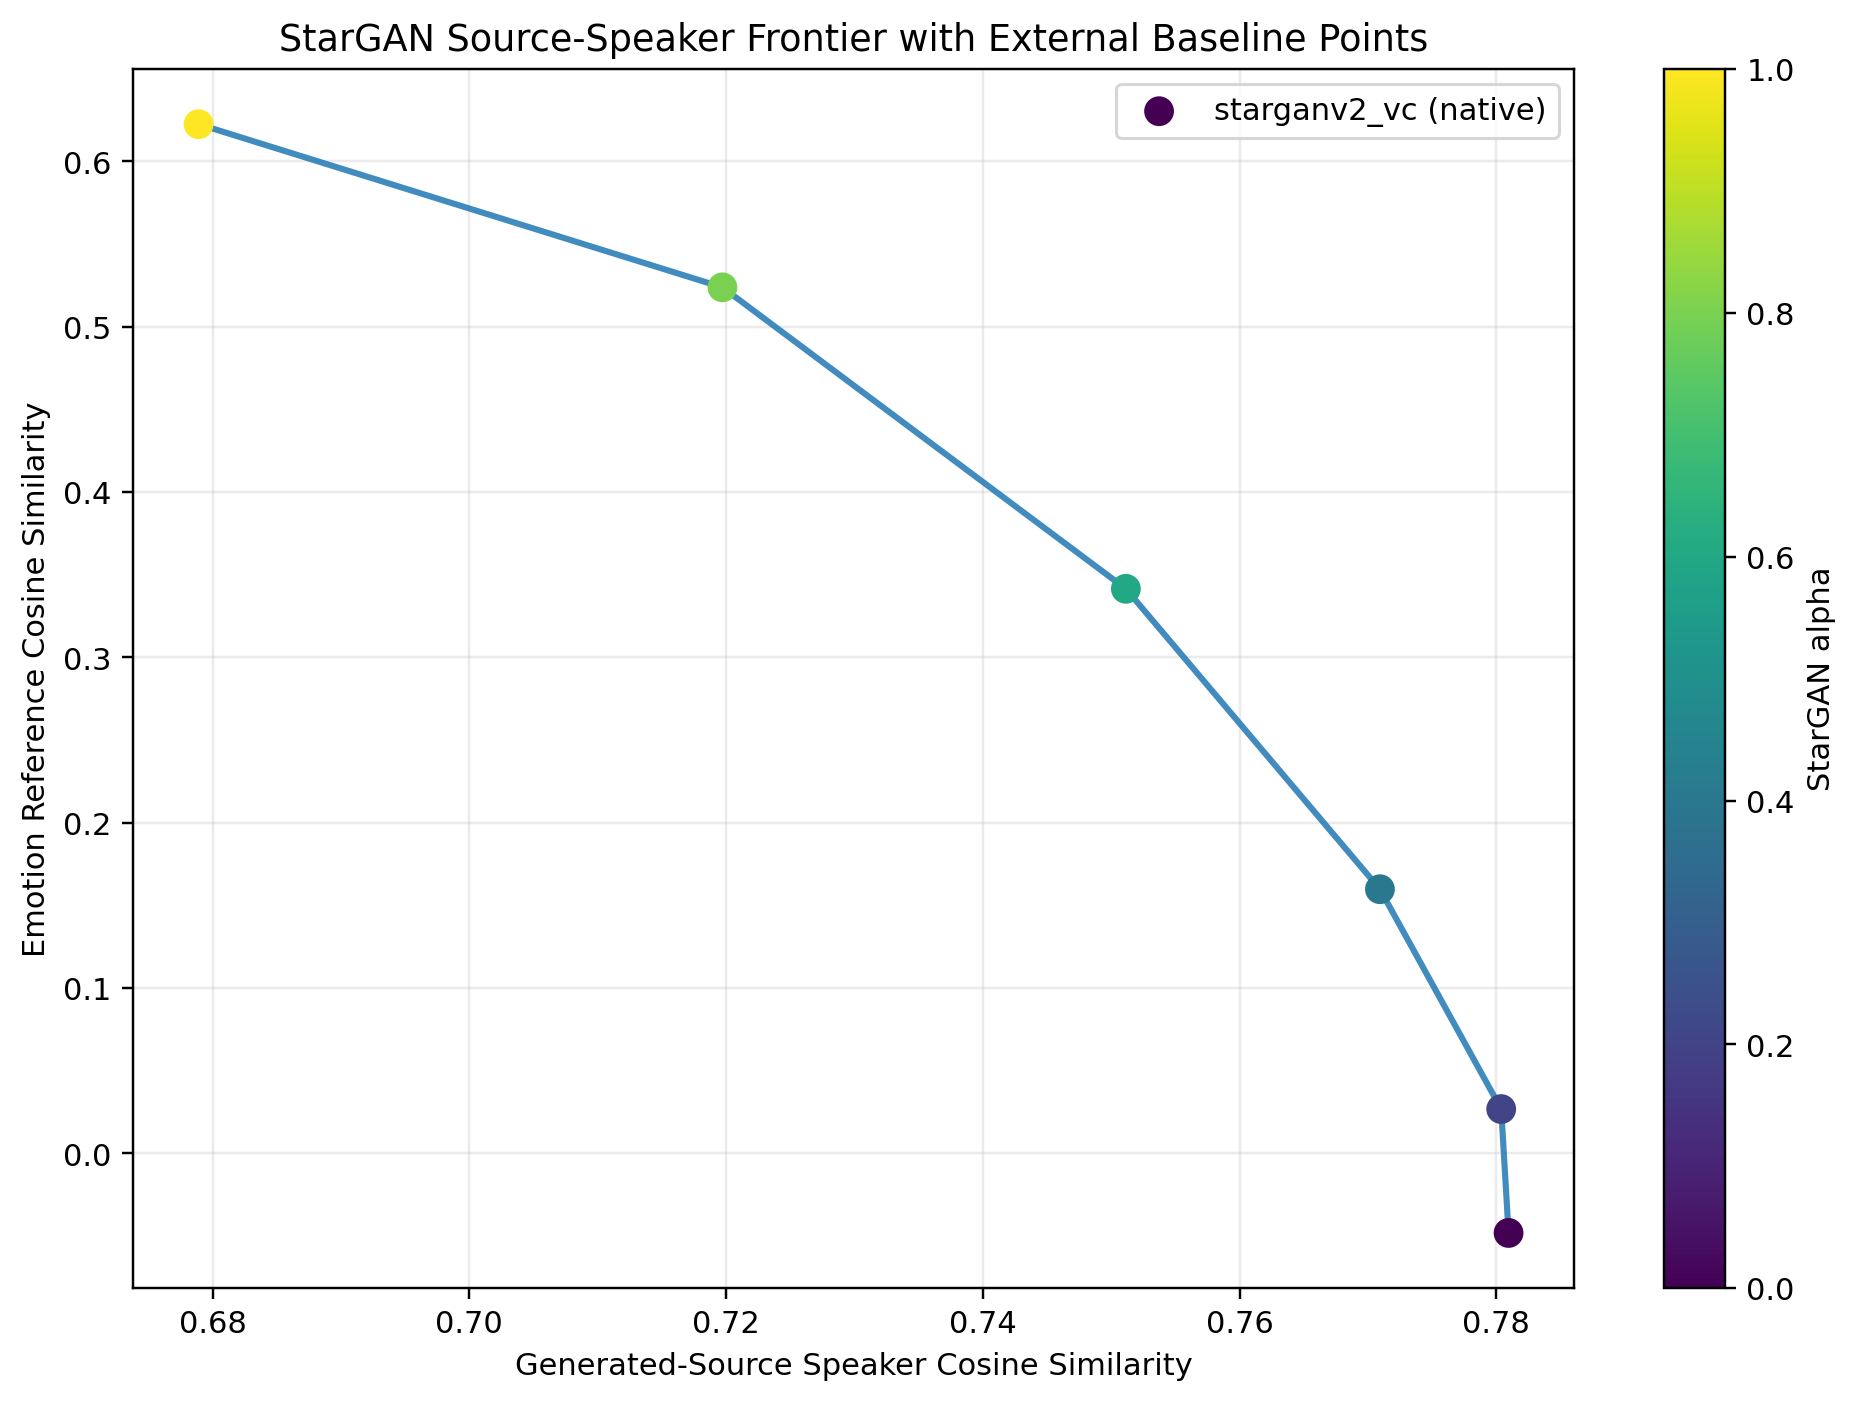
\includegraphics[width=\linewidth]{figures/frontier_native_esd_ssst.png}\\
\small (a) ESD SSST
\end{minipage}\hfill
\begin{minipage}{0.48\textwidth}
\centering
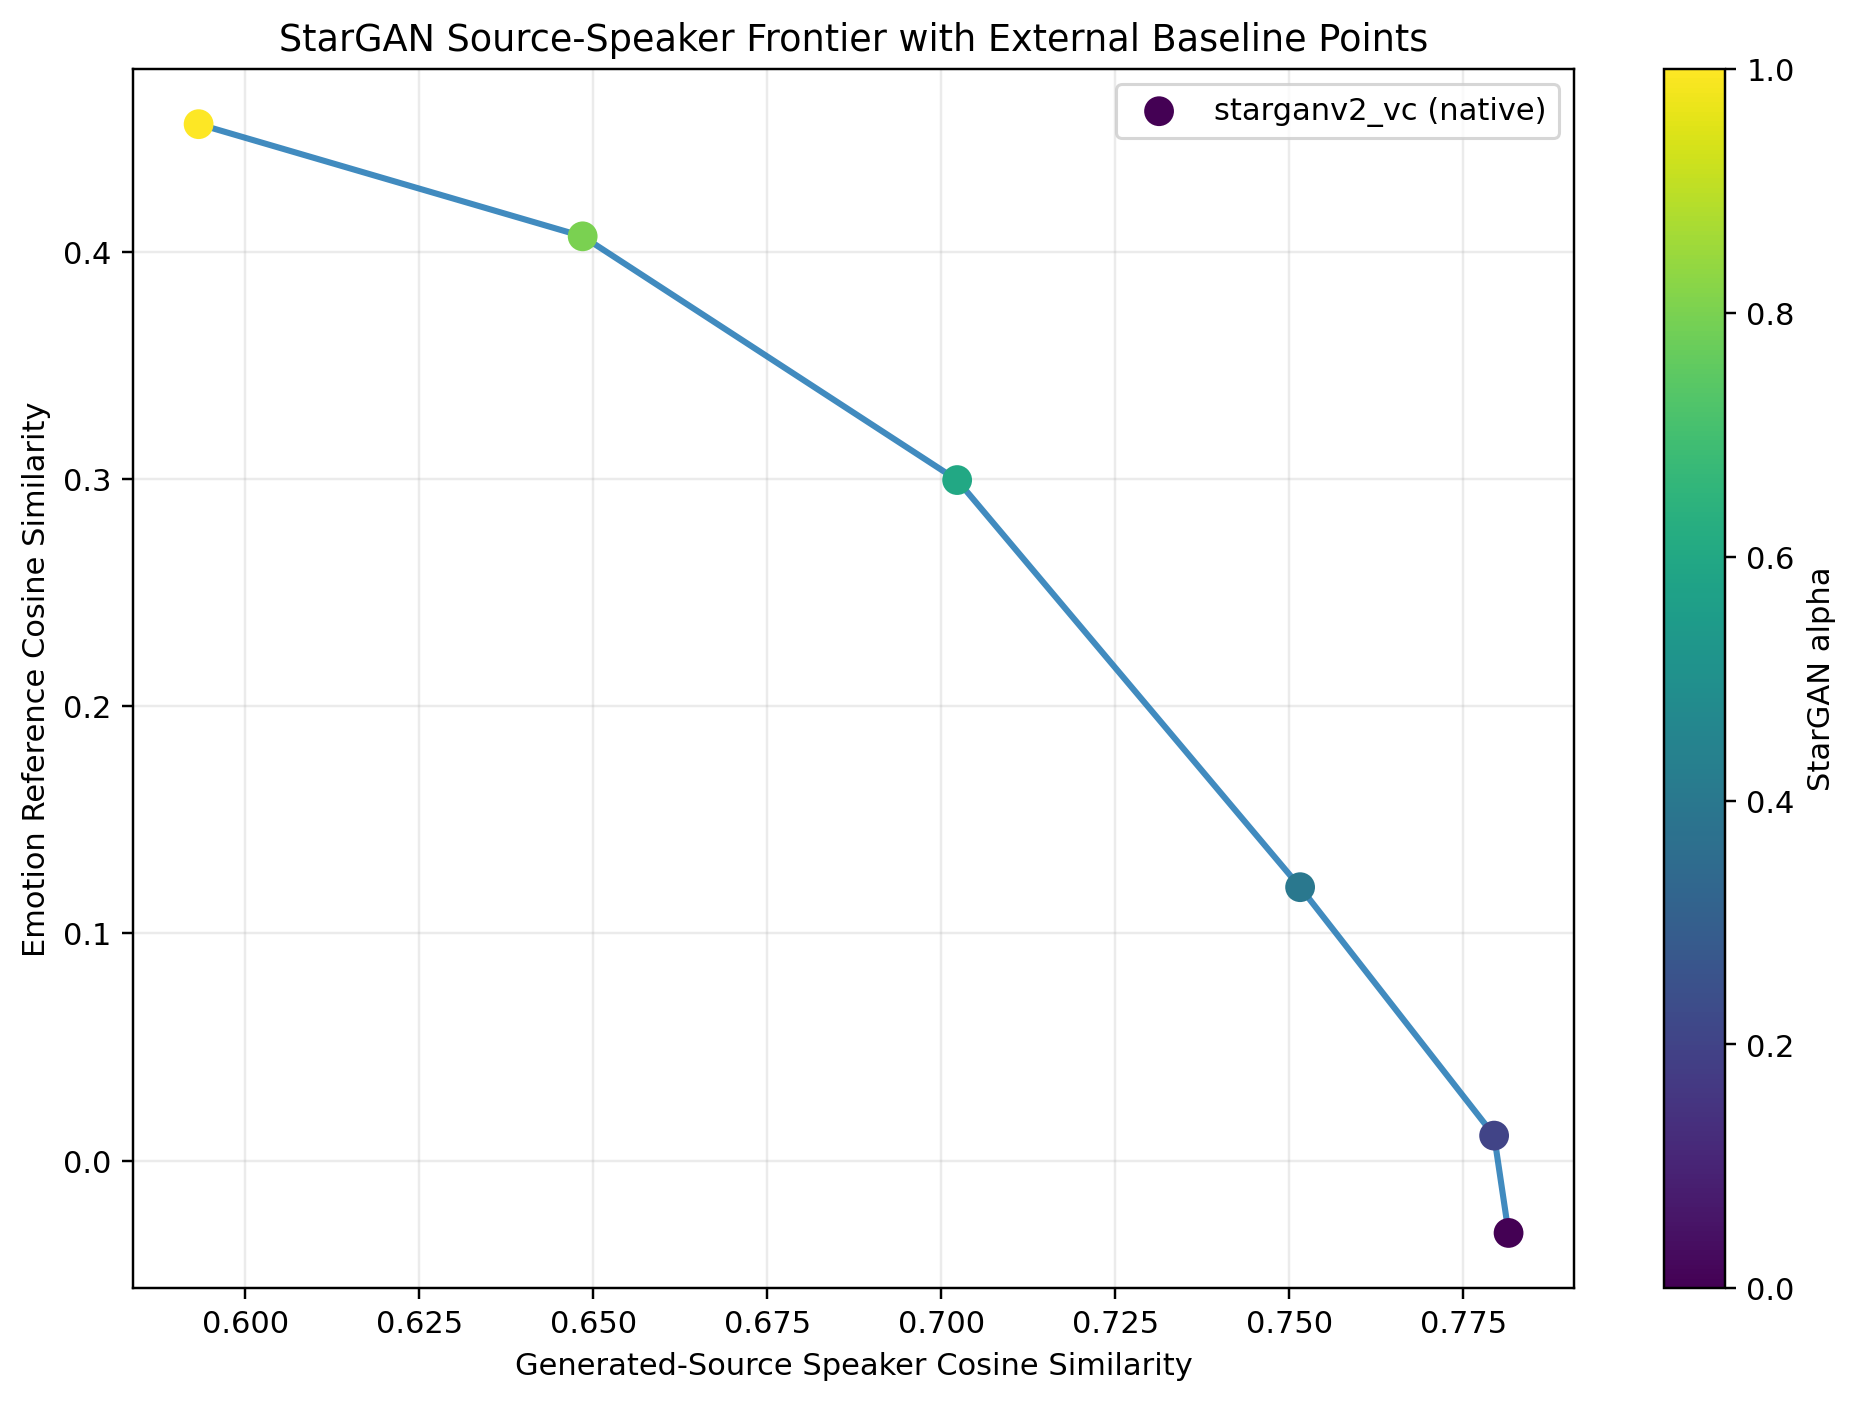
\includegraphics[width=\linewidth]{figures/frontier_native_esd_dsst.png}\\
\small (b) ESD DSST
\end{minipage}
\caption{Native-intensity source-speaker frontiers on ESD. Increasing alpha strengthens target-emotion alignment but reduces generated-source speaker similarity, with a larger speaker-preservation cost in DSST than in SSST.}
\label{fig:endpoint-tradeoff}
\end{figure*}

\begin{table*}[t]
\caption{Overall objective evaluation metrics for the propsed baselines, for each metric we record $\alpha=0$, $\alpha=1$, and $\Delta =\alpha_1-\alpha_0$. Emotion-side metrics show clear improvements with increasing $\alpha$, while speaker-side metrics show a consistent drop, especially in the DSST setting.}
\label{tab:endpoint-summary}
\centering
\tiny
\resizebox{\textwidth}{!}{%
\begin{tabular}{ll*{12}{r}}
\toprule
Model & Dataset &
\multicolumn{3}{c}{$\mathrm{ACC}_{\mathrm{emo}}$} &
\multicolumn{3}{c}{$\mathrm{CONF}_{\mathrm{emo}}$} &
\multicolumn{3}{c}{$\mathrm{SIM}_{\mathrm{emo}}$} &
\multicolumn{3}{c}{$\mathrm{SIM}_{\mathrm{spk-src}}$} \\
\cmidrule(lr){3-5}\cmidrule(lr){6-8}\cmidrule(lr){9-11}\cmidrule(lr){12-14}
 & & $\alpha_0$ & $\alpha_1$ & $\Delta$ & $\alpha_0$ & $\alpha_1$ & $\Delta$ & $\alpha_0$ & $\alpha_1$ & $\Delta$ & $\alpha_0$ & $\alpha_1$ & $\Delta$ \\
\midrule
StarGANv2-IEVC  & ESD SSST & 0.194 & 0.664 & 0.470 & 0.192 & 0.660 & 0.468 & -0.037 & 0.602 & 0.639 & 0.780 & 0.683 & -0.097 \\
CycleGAN-IEVC & ESD SSST & 0.208 & 0.481 & 0.274 & 0.207 & 0.482 & 0.275 & 0.012 & 0.418 & 0.406 & 0.876 & 0.730 & -0.146 \\
\\
StarGANv2-NEVC (proposed)  & ESD SSST & 0.190 & 0.654 & 0.464 & 0.191 & 0.653 & 0.462 & -0.048 & \textbf{0.623} & 0.671 & 0.781 & 0.679 & -0.102 \\
StarGANv2-NEVC w/ Speaker-Classifier & ESD SSST & 0.191 & \textbf{0.674} & 0.482 & 0.192 & \textbf{0.673} & 0.481 & -0.054 & 0.606 & 0.660 & 0.783 & 0.714 & \textbf{-0.069} \\
StarGANv2-NEVC w/ Speaker-Contrastive & ESD SSST & 0.182 & 0.506 & 0.324 & 0.183 & 0.506 & 0.323 & -0.077 & 0.429 & 0.506 & 0.821 & \textbf{0.746} & -0.075 \\
\midrule
StarGANv2-IEVC & ESD DSST & 0.201 & 0.544 & 0.343 & 0.202 & 0.545 & 0.344 & -0.021 & 0.481 & 0.502 & 0.783 & 0.592 & -0.191 \\
CycleGAN-IEVC & ESD DSST & 0.058 & \textbf{0.642} & 0.583 & 0.059 & \textbf{0.640} & 0.581 & -0.156 & \textbf{0.500} & 0.656 & 1.000 & 0.706 & -0.294 \\
\\
StarGANv2-NEVC & ESD DSST & 0.190 & 0.515 & 0.325 & 0.191 & 0.514 & 0.323 & -0.032 & 0.456 & 0.488 & 0.782 & 0.593 & -0.188 \\
StarGANv2-NEVC w/ Speaker-Classifier & ESD DSST & 0.215 & 0.552 & 0.337 & 0.215 & 0.550 & 0.335 & -0.019 & 0.470 & 0.489 & 0.783 & 0.673 & -0.110 \\
StarGANv2-NEVC w/ Speaker-Contrastive & ESD DSST & 0.220 & 0.388 & 0.168 & 0.218 & 0.382 & 0.163 & -0.021 & 0.321 & 0.342 & 0.822 & \textbf{0.746} & \textbf{-0.076} \\
\midrule
StarGANv2-IEVC & CREMA-D & 0.280 & 0.259 & -0.021 & 0.278 & 0.258 & -0.019 & 0.291 & 0.318 & 0.027 & 0.302 & 0.302 & 0.000 \\
CycleGAN-IEVC & CREMA-D & 0.304 & \textbf{0.553} & 0.249 & 0.304 & \textbf{0.549} & 0.245 & 0.323 & 0.426 & 0.103 & 0.719 & 0.392 & -0.327 \\
\\
StarGANv2-NEVC w/ Speaker-Classifier & CREMA-D & 0.336 & 0.457 & 0.121 & 0.334 & 0.454 & 0.120 & 0.308 & \textbf{0.471} & 0.163 & 0.460 & \textbf{0.461} & \textbf{0.001} \\

\bottomrule
\end{tabular}
}
\end{table*}

Figure~\ref{fig:endpoint-tradeoff} and Table~\ref{tab:endpoint-summary} show the general frontier pattern.
Across ESD SSST, both StarGANv2-IEVC and StarGANv2-NEVC increase target-emotion scores as alpha moves from 0 to 1, but both lose source-speaker similarity.
StarGANv2-IEVC raises $\mathrm{ACC}_{\mathrm{emo}}$ from 0.194 to 0.664 and $\mathrm{SIM}_{\mathrm{emo}}$ from -0.037 to 0.602, while $\mathrm{SIM}_{\mathrm{spk-src}}$ drops from 0.780 to 0.683.
StarGANv2-NEVC follows the same frontier direction, with $\mathrm{ACC}_{\mathrm{emo}}$ rising from 0.190 to 0.654 and $\mathrm{SIM}_{\mathrm{spk-src}}$ falling from 0.781 to 0.679.
The speaker-classifier branch gives the best SSST alpha-1 target-class score and the smallest SSST speaker delta, but its emotion-reference cosine is lower than the proposed NEVC row.

The DSST setting makes the tradeoff more severe and exposes stronger model differences.
CycleGAN-IEVC has the largest alpha-1 emotion scores on DSST, reaching 0.642 $\mathrm{ACC}_{\mathrm{emo}}$, but it also has the largest speaker drop, -0.294.
The contrastive NEVC branch has the strongest DSST speaker preservation at alpha 1, 0.746, and the smallest absolute speaker delta, -0.076, but its emotion accuracy is only 0.388.
This is the clearest table-level evidence for the core claim: the model that looks best by target emotion is not the model that best preserves source-speaker identity.
Thus the relevant result is not a single endpoint, but the shape and location of the emotion--speaker operating point.

\subsection{Per-Dataset Evidence}

\begin{figure*}[t]
\centering
\begin{minipage}{0.48\textwidth}
\centering
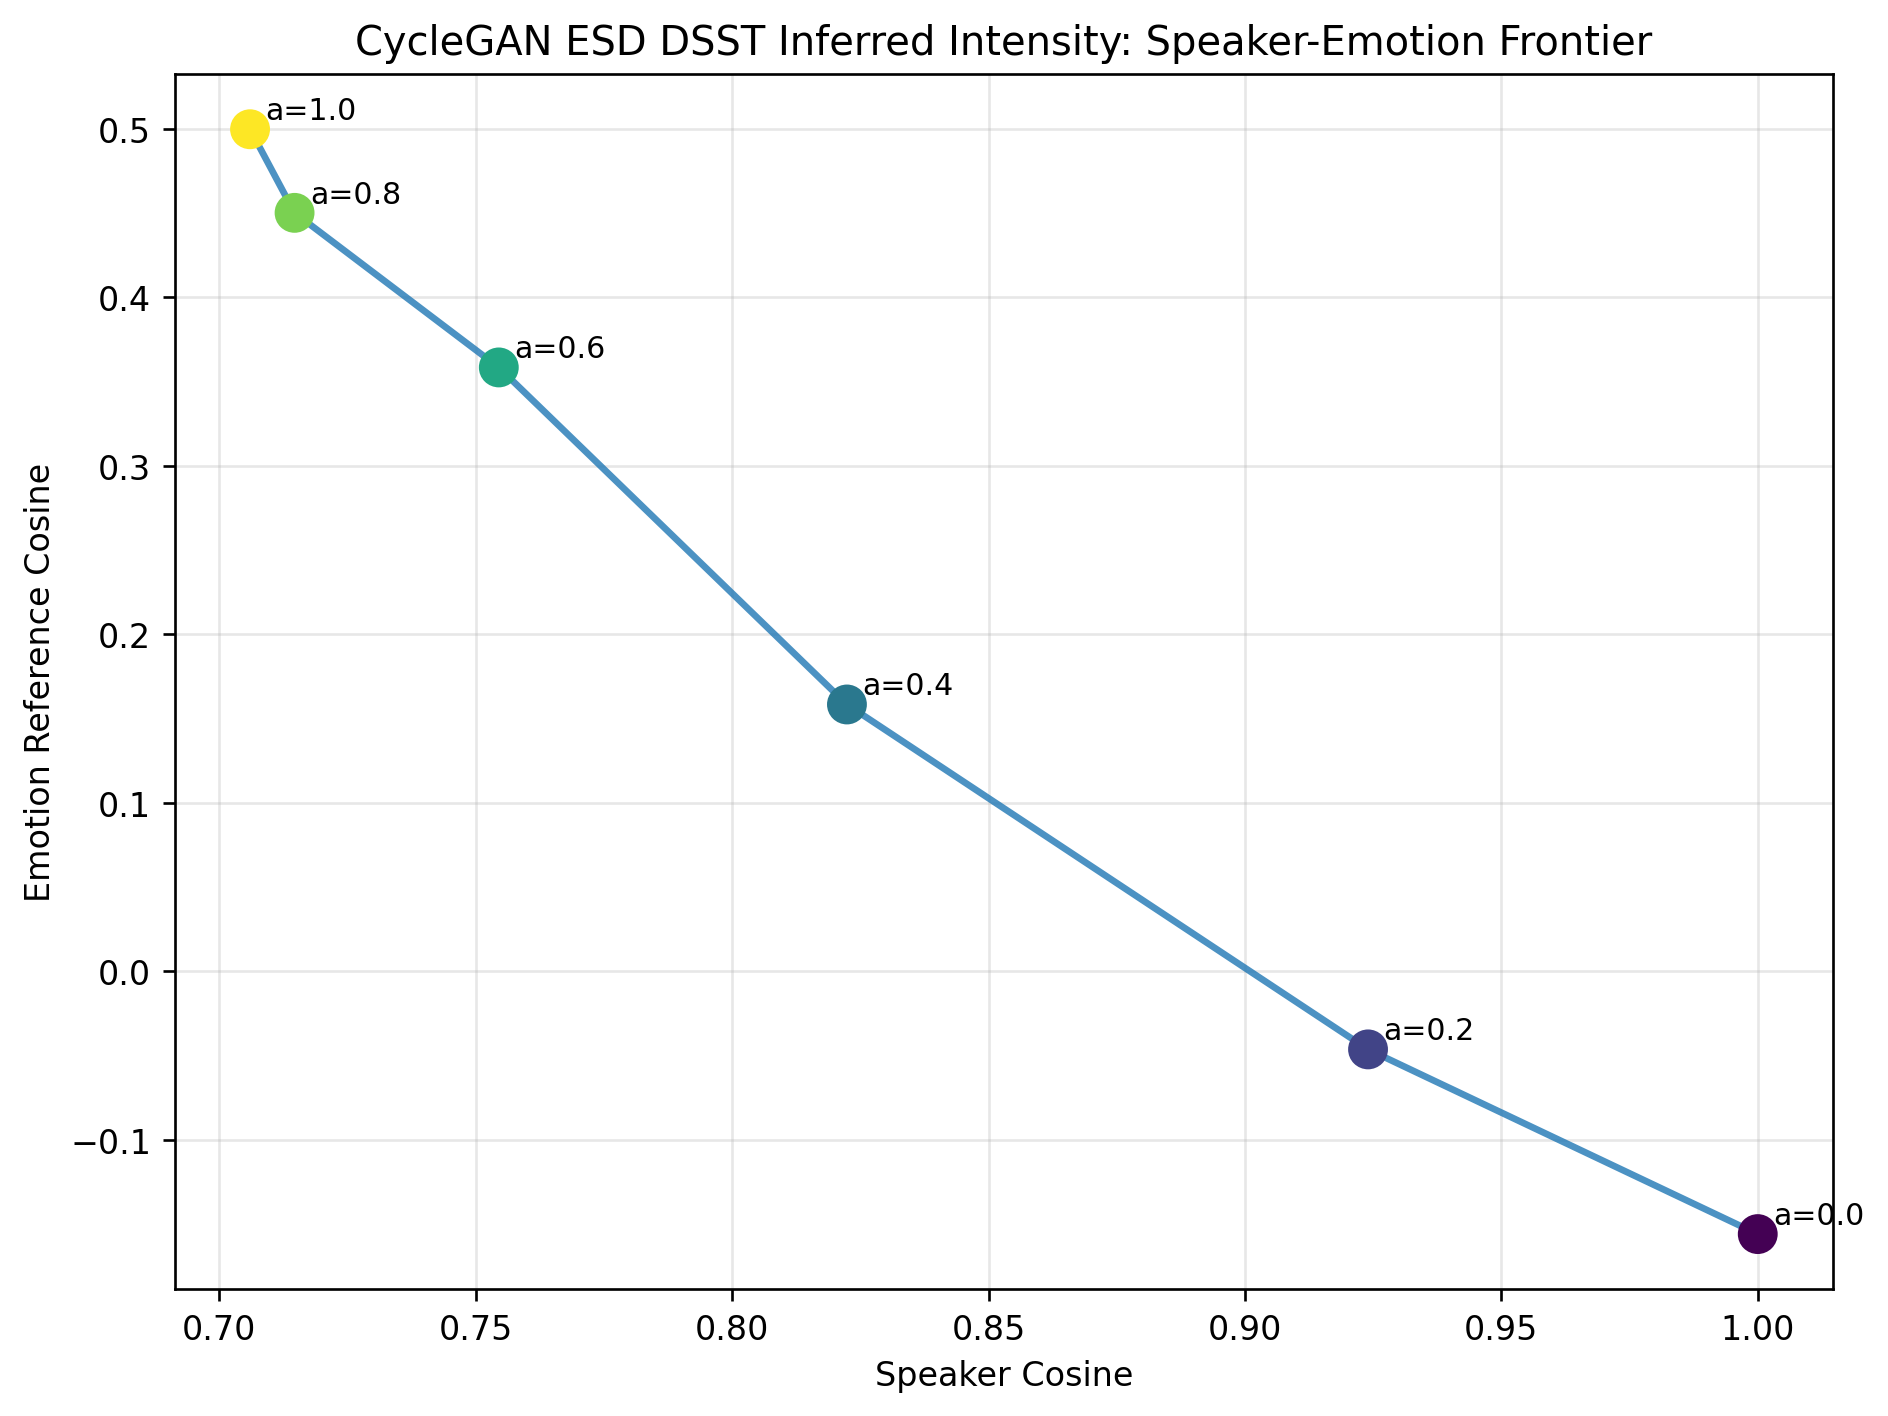
\includegraphics[width=\linewidth]{figures/frontier_cyclegan_esd_dsst.png}\\
\small (a) CycleGAN, ESD DSST
\end{minipage}\hfill
\begin{minipage}{0.48\textwidth}
\centering
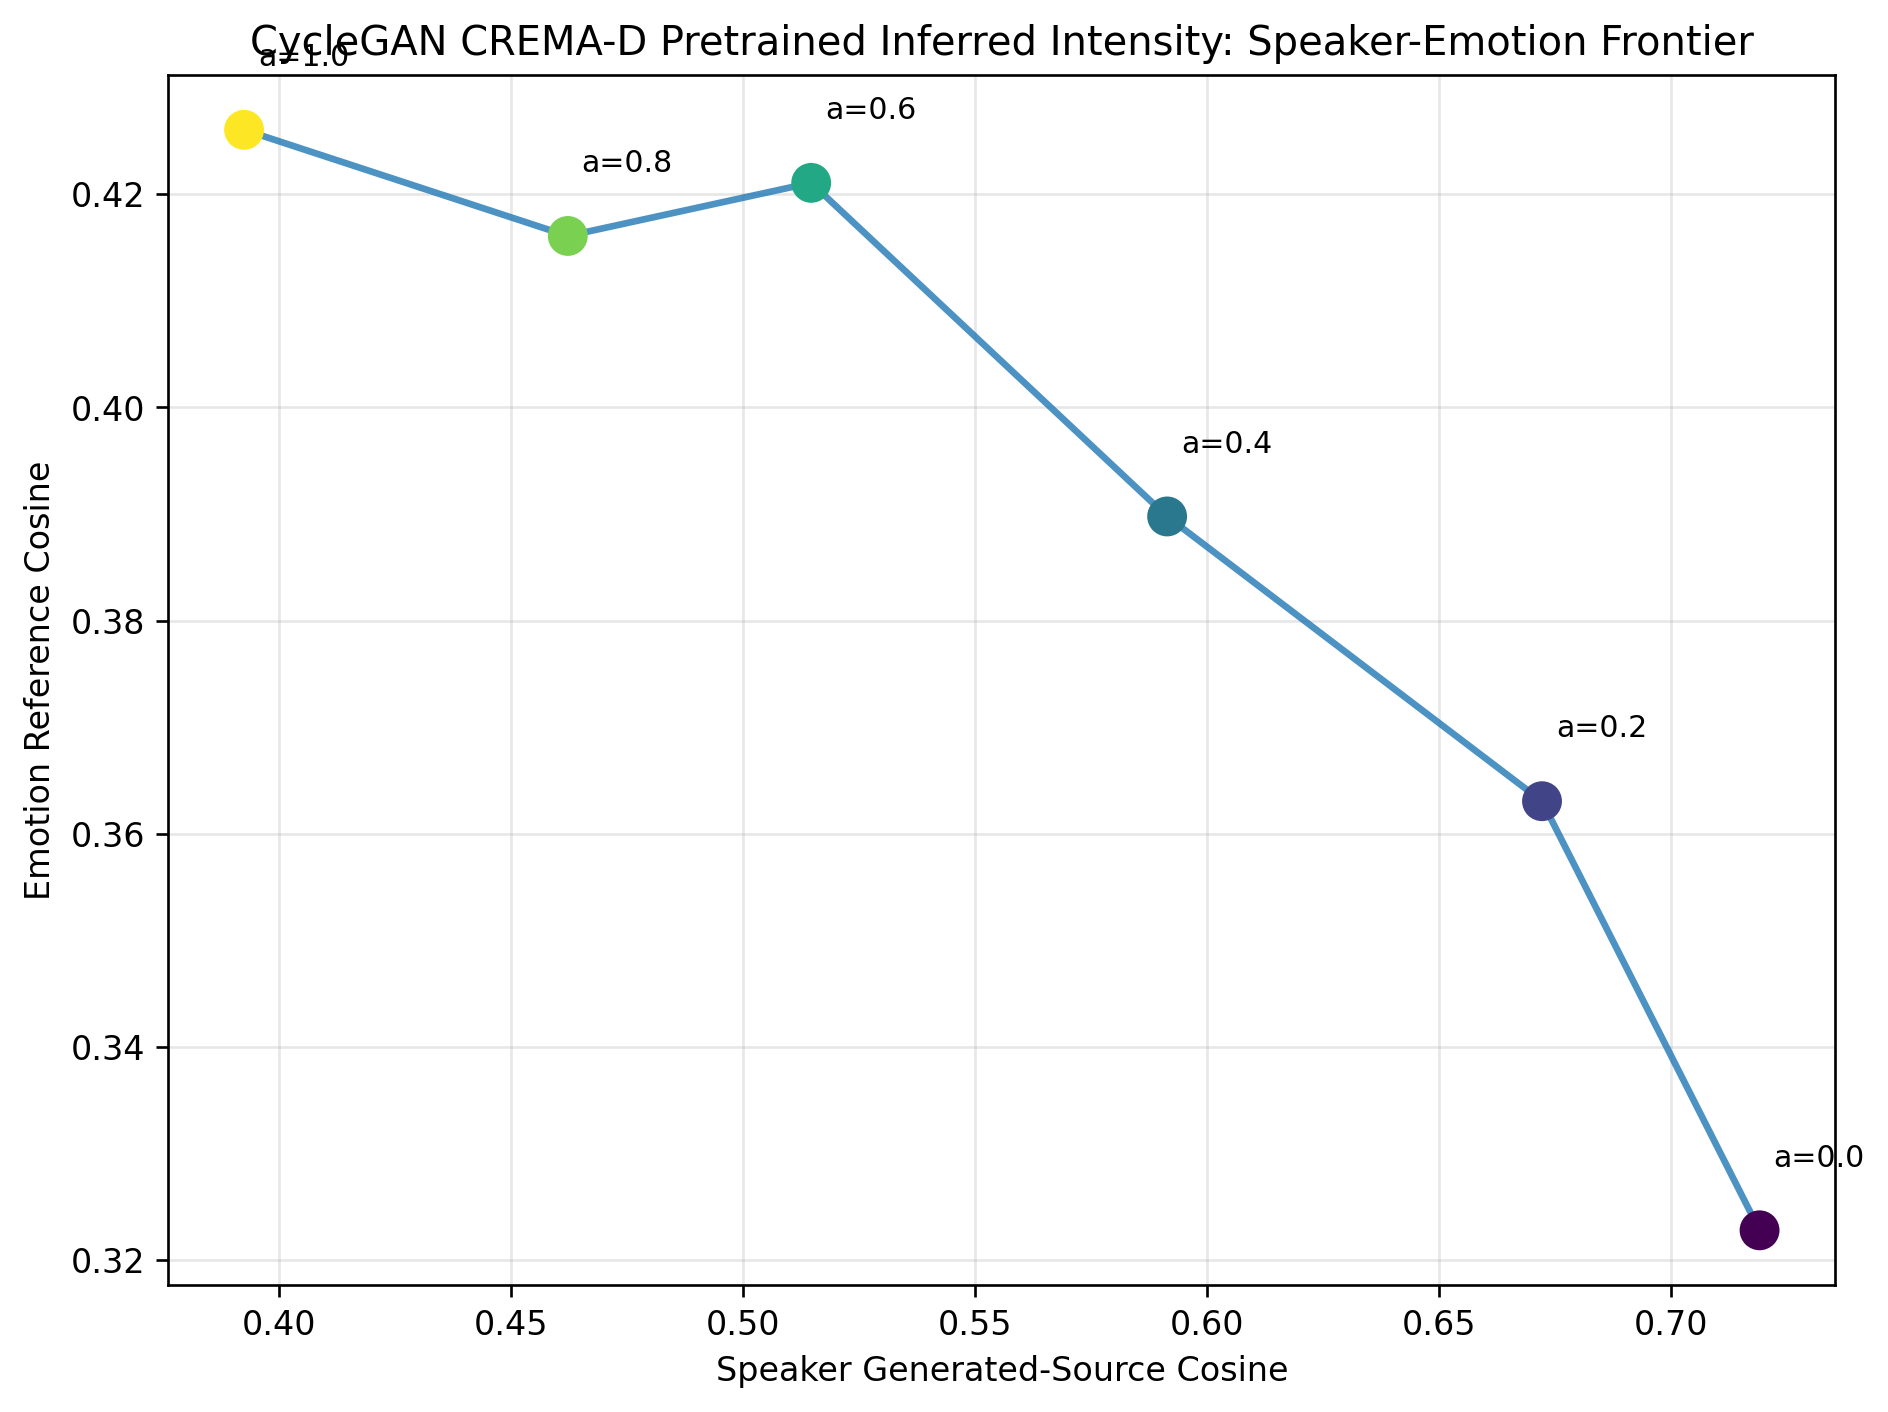
\includegraphics[width=\linewidth]{figures/frontier_cyclegan_cremad_from_scratch.png}\\
\small (b) CycleGAN, CREMA-D from scratch
\end{minipage}
\caption{CycleGAN spectrum-conversion frontiers. CycleGAN reaches strong target-emotion endpoints, but the curves occupy a higher-drift region than the StarGAN-style intensity sweeps.}
\label{fig:cyclegan-frontier}
\end{figure*}

\begin{figure*}[t]
\centering
\begin{minipage}{0.48\textwidth}
\centering
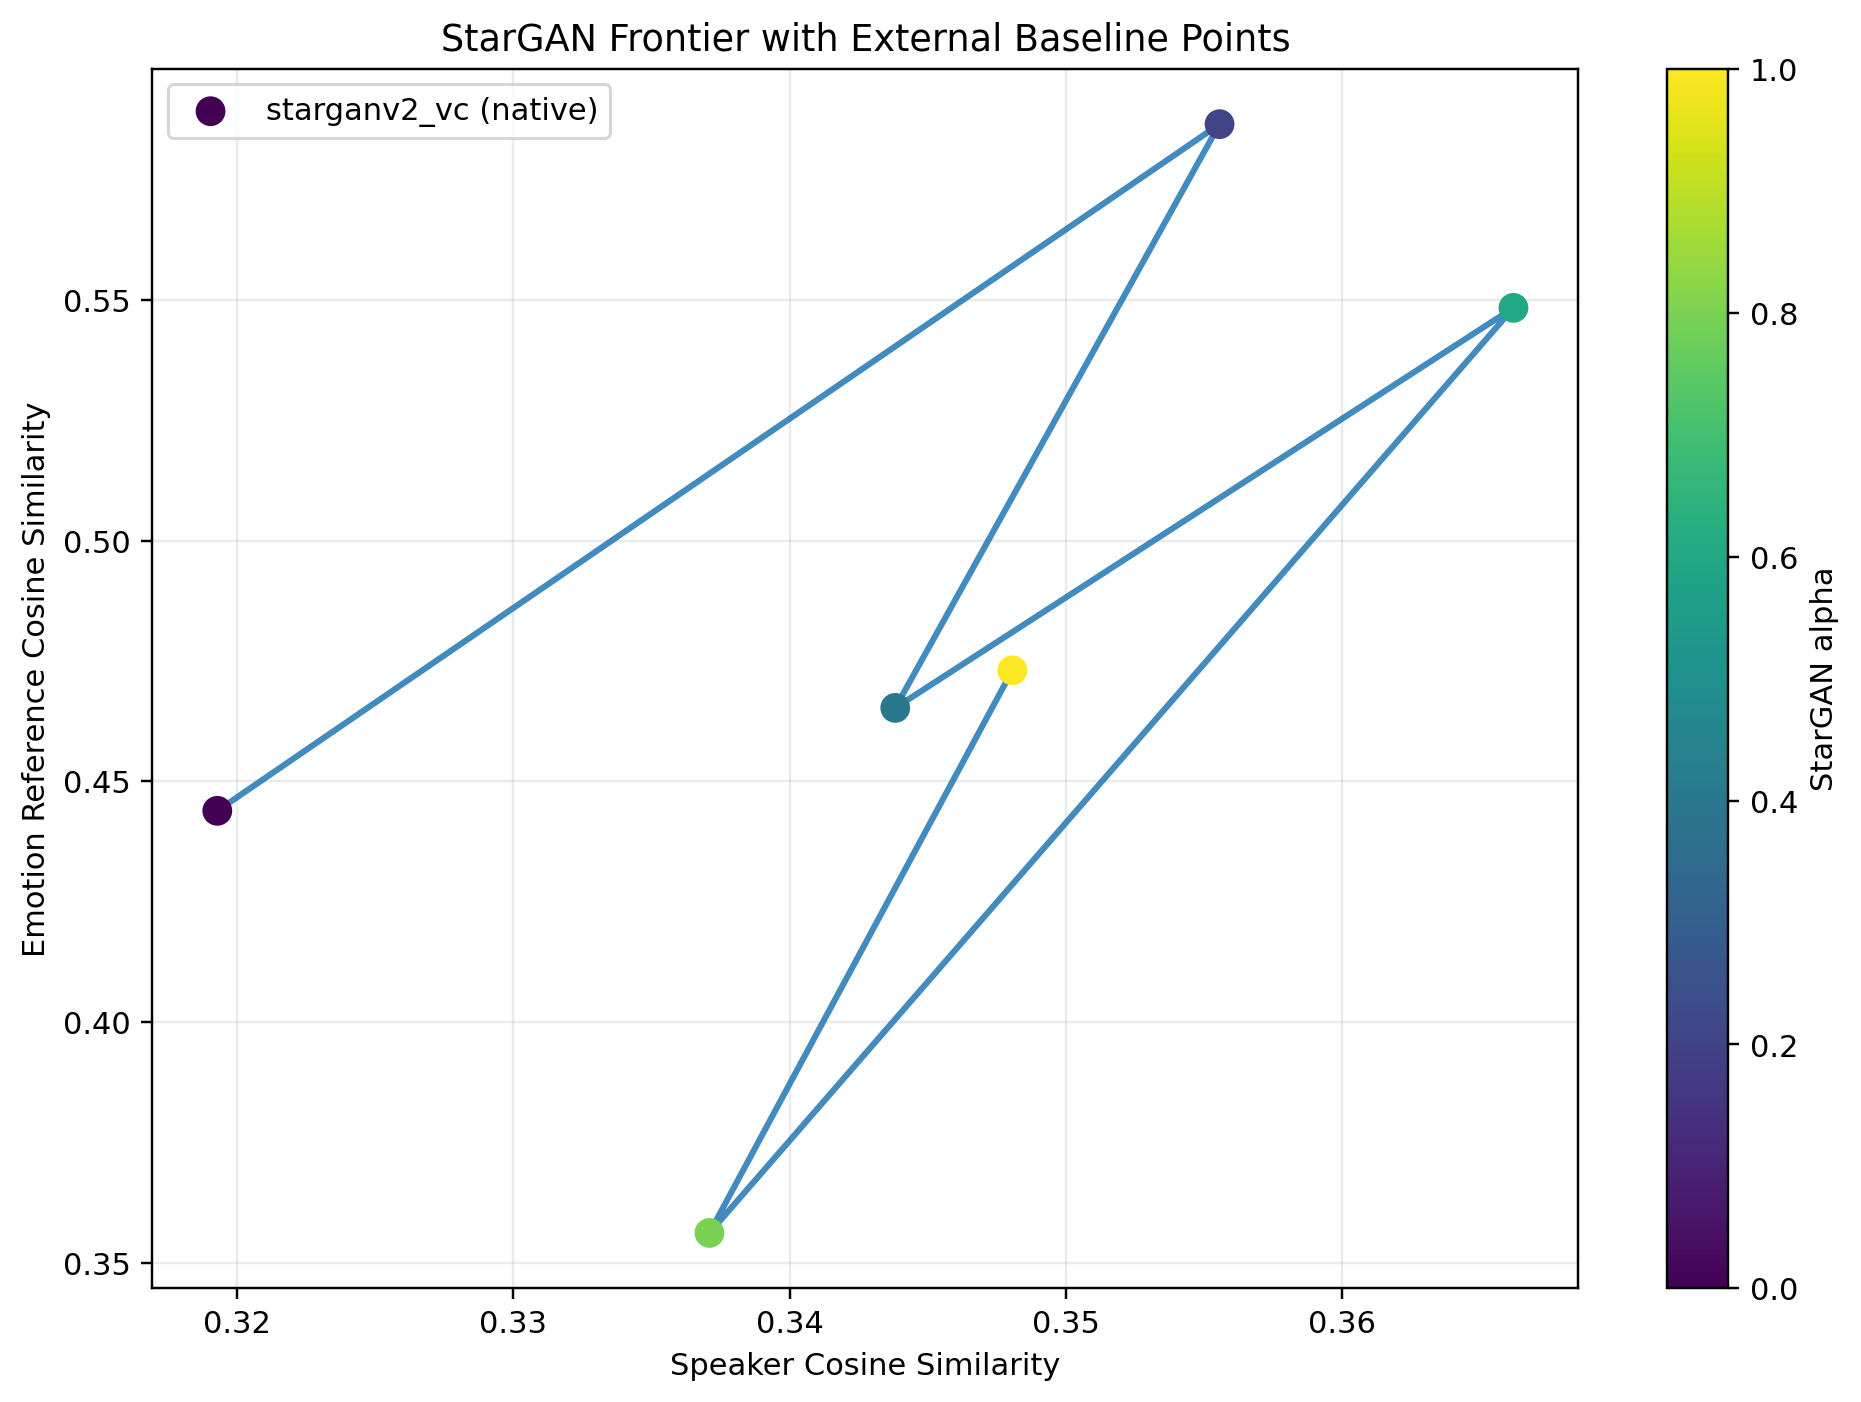
\includegraphics[width=\linewidth]{figures/frontier_native_cremad_from_scratch_epoch30.png}\\
\small (a) Native ranker, epoch 30
\end{minipage}\hfill
\begin{minipage}{0.48\textwidth}
\centering
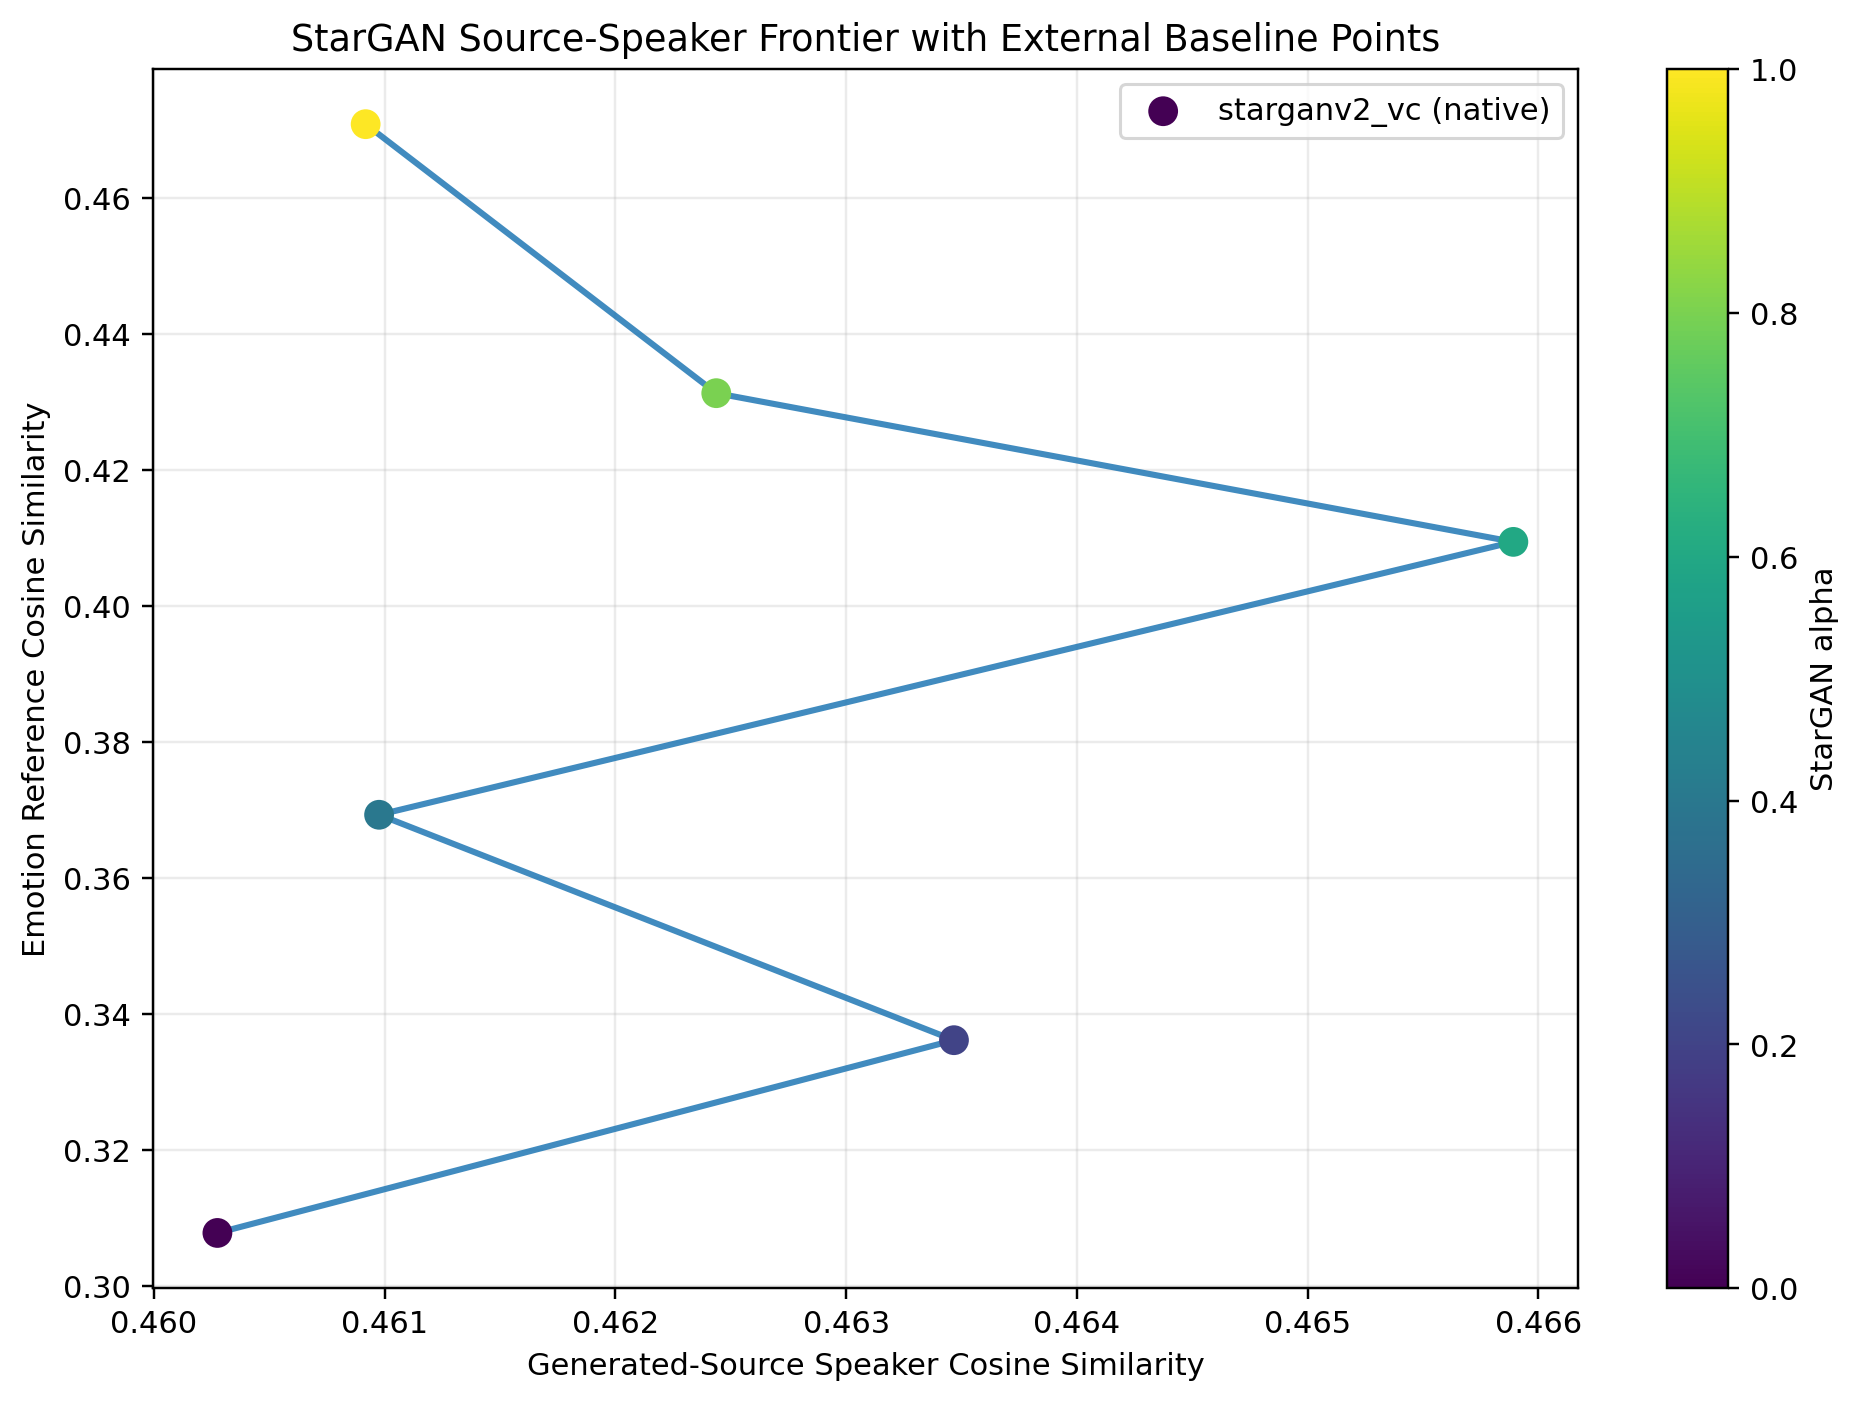
\includegraphics[width=\linewidth]{figures/frontier_ablation_speaker_cls_cremad_from_scratch.png}\\
\small (b) Speaker-classifier branch
\end{minipage}
\caption{CREMA-D from-scratch frontiers. The from-scratch condition is a stress test: the native ranker is unstable and emotion-specific, while the speaker-classifier branch is the strongest StarGAN-style from-scratch condition.}
\label{fig:cremad-from-scratch}
\end{figure*}

The dataset-level evidence has two different roles.
ESD is the main frontier evidence because both SSST and DSST produce structured alpha curves with clear emotion gains and measurable speaker losses.
CREMA-D from scratch is not a clean replication of the ESD pattern; it is a stress test for whether the same evaluation exposes unstable or dataset-dependent behavior.
In Table~\ref{tab:endpoint-summary}, CycleGAN-IEVC reaches the highest CREMA-D emotion accuracy at alpha 1, 0.553, but its source-speaker cosine falls sharply from 0.719 to 0.392.
By contrast, the speaker-classifier StarGANv2-NEVC row reaches lower alpha-1 accuracy, 0.457, but has the best CREMA-D source-speaker cosine at alpha 1, 0.461, and almost no speaker delta.

Figure~\ref{fig:cyclegan-frontier} shows why CycleGAN is useful as a baseline.
It occupies high-emotion, high-drift regions: this is especially visible on DSST and CREMA-D, where emotion scores can be strong while source-speaker preservation degrades substantially.
Figure~\ref{fig:cremad-from-scratch} shows the complementary StarGAN-style result.
The speaker-classifier branch is the more stable CREMA-D from-scratch operating point, improving emotion-reference similarity while keeping source-speaker cosine nearly unchanged.
The conclusion is therefore bounded: CREMA-D does not prove a universal frontier shape, but it shows that the proposed evaluation can distinguish high-emotion/high-drift systems from more speaker-stable operating points.

\subsection{Per-Emotion Evidence}

\begin{figure}[t]
\centering
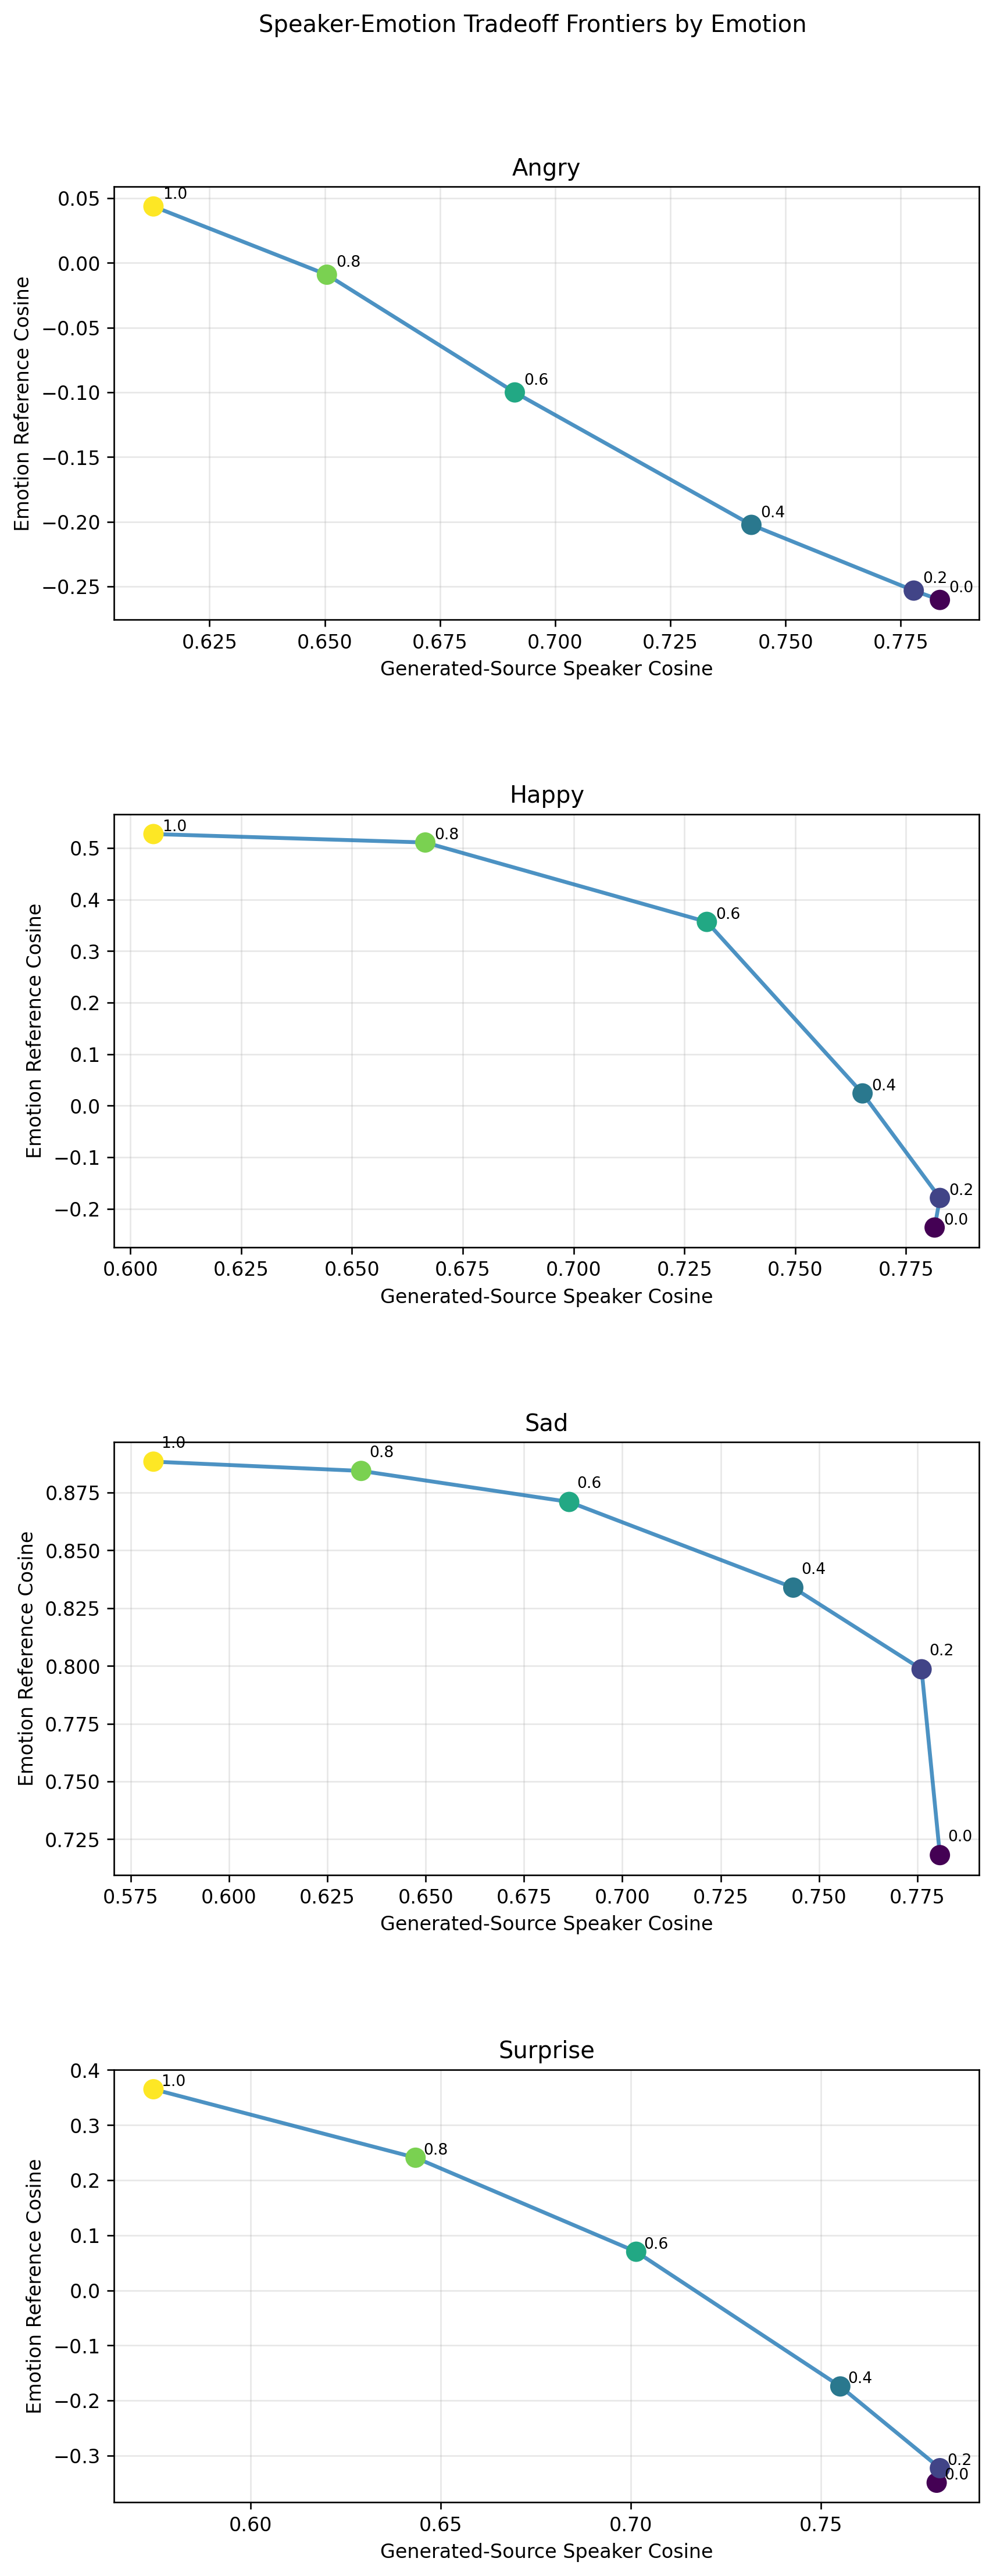
\includegraphics[height=0.82\textheight]{figures/frontier_per_emotion_native_esd_dsst.png}
\caption{Per-emotion native-intensity frontiers on ESD DSST. Sad reaches high target-emotion accuracy with a stable curve, while angry and surprise remain weak and are easy to overstate in aggregate metrics.}
\label{fig:per-emotion-frontier}
\end{figure}

\begin{table}[t]
\caption{Alpha-1 per-emotion accuracy on ESD DSST.}
\label{tab:per-emotion-dsst}
\centering
\footnotesize
\begin{tabular}{lrrrr}
\toprule
System & Angry & Happy & Sad & Surprise \\
\midrule
StarGANv2-IEVC & 0.167 & 0.652 & 0.996 & 0.359 \\
StarGANv2-NEVC & 0.163 & 0.685 & 0.996 & 0.215 \\
StarGANv2-NEVC-Spk-Cls & 0.244 & 0.652 & 0.996 & 0.315 \\
StarGANv2-NEVC-Spk-Con  & 0.040 & 0.468 & 1.000 & 0.033 \\
\bottomrule
\end{tabular}
\end{table}

Figure~\ref{fig:per-emotion-frontier} and Table~\ref{tab:per-emotion-dsst} show that aggregate curves hide large label differences.
For native intensity on ESD DSST, sad reaches 0.996 accuracy and happy reaches 0.685, but angry and surprise remain much weaker at 0.163 and 0.215.
The speaker-classifier branch improves the weak labels somewhat, reaching 0.244 for angry and 0.315 for surprise, while keeping sad at 0.996.
The contrastive branch exposes the opposite failure mode: it preserves speakers well but collapses difficult emotion transfer, with angry and surprise falling to 0.040 and 0.033.
The conclusion is that the tradeoff is not uniform across emotions; per-emotion plots are necessary to prevent sad-dominated aggregate scores from overstating controllability.

\subsection{Model Comparisons and Significance}

\begin{figure*}[t]
\centering
\begin{minipage}{0.48\textwidth}
\centering
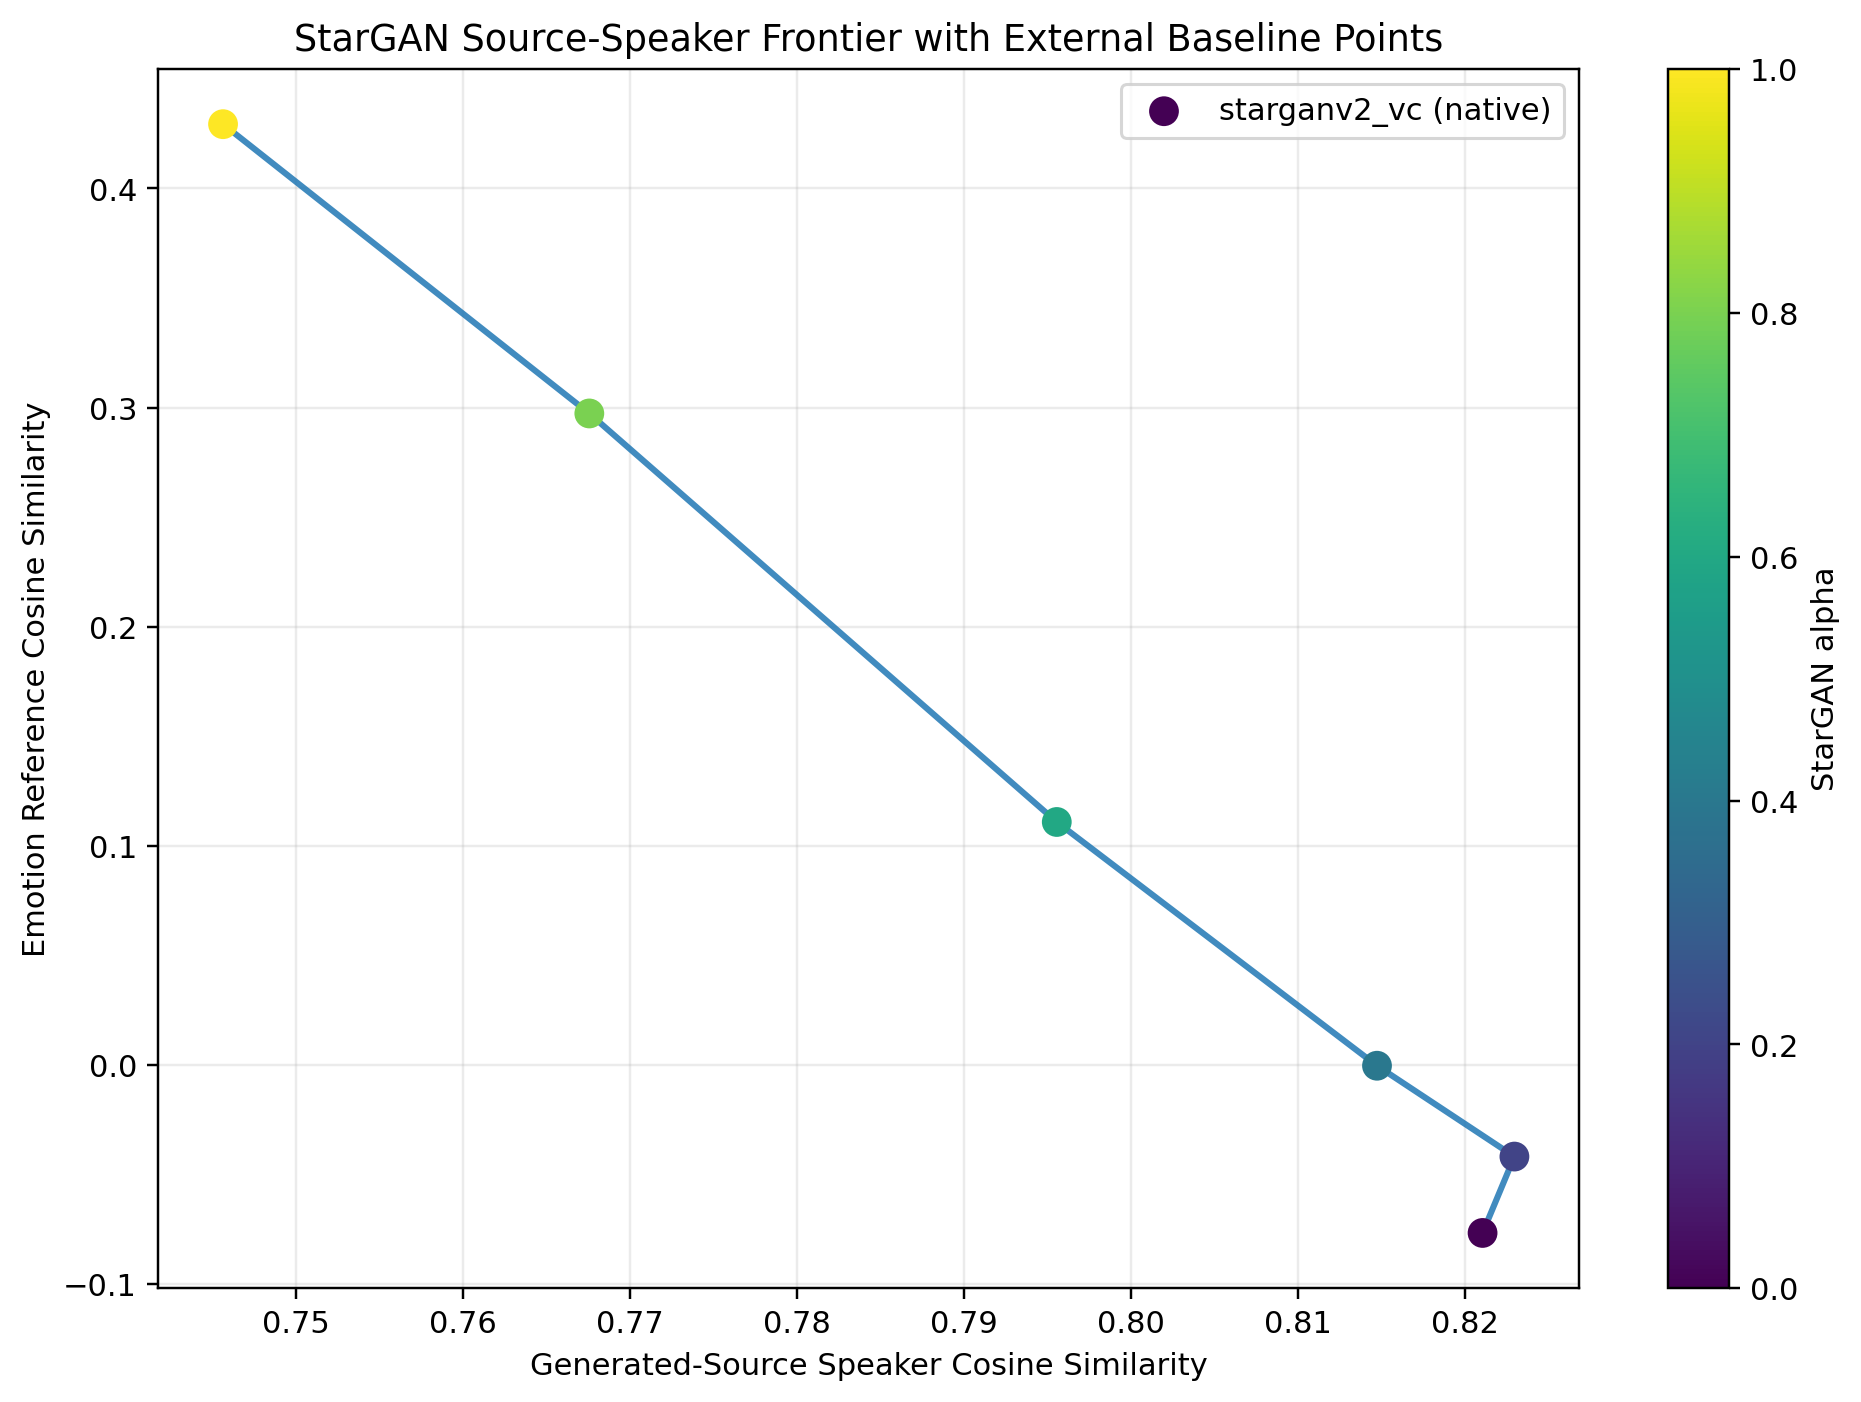
\includegraphics[width=\linewidth]{figures/frontier_ablation_speaker_contrastive_esd_ssst.png}\\
\small (a) Contrastive branch, ESD SSST
\end{minipage}\hfill
\begin{minipage}{0.48\textwidth}
\centering
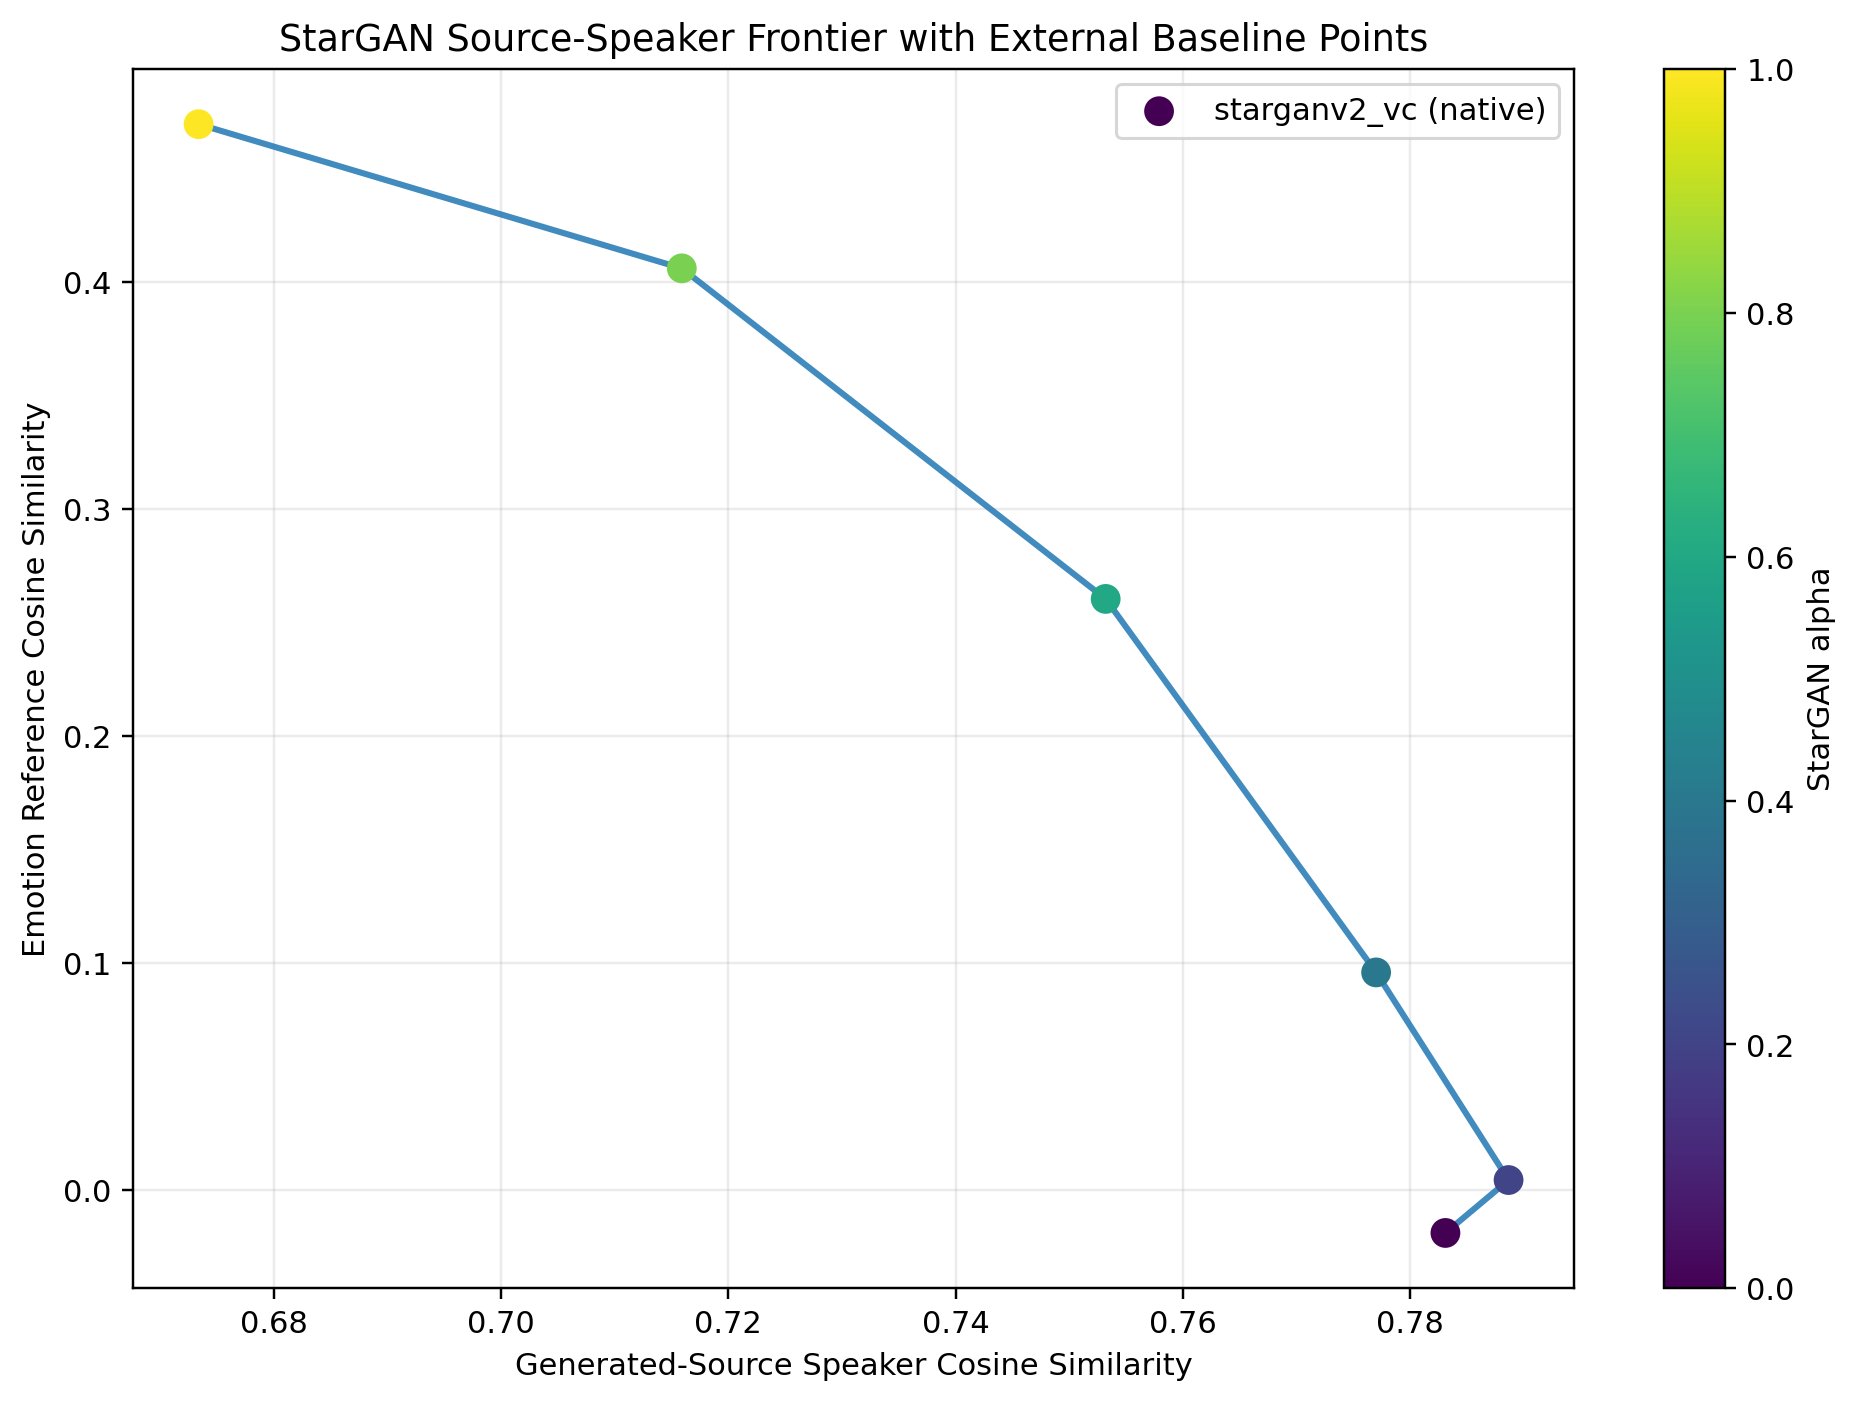
\includegraphics[width=\linewidth]{figures/frontier_ablation_speaker_cls_esd_dsst.png}\\
\small (b) Speaker-classifier branch, ESD DSST
\end{minipage}
\caption{Speaker-related ablation frontiers on ESD. The contrastive branch shifts toward speaker preservation at the cost of target-emotion transfer. The speaker-classifier branch is more favorable on DSST, but still has metric-specific tradeoffs.}
\label{fig:ablation-frontier}
\end{figure*}

\begin{table*}[t]
\caption{Selected paired significance tests for model comparisons. $\Delta$ is left model minus right model. Positive is favorable for accuracy, emotion-reference cosine, and speaker cosine; negative is favorable for MCD.}
\label{tab:significance}
\centering
\scriptsize
\begin{tabular}{llrrrrp{0.24\textwidth}}
\toprule
Setting & Comparison and metric & Left & Right & $\Delta$ & 95\% CI & Interpretation \\
\midrule
SSST & Spk-cls. vs native, speaker cosine & 0.761 & 0.747 & 0.014 & [0.013, 0.016] & Significant speaker gain; $q<10^{-66}$. \\
SSST & Spk-cls. vs native, emotion acc. & 0.405 & 0.401 & 0.004 & [-0.007, 0.014] & No significant accuracy change. \\
SSST & Spk-cls. vs native, emotion-ref. & 0.259 & 0.271 & -0.012 & [-0.022, -0.003] & Significant emotion-reference loss; $q<10^{-5}$. \\
\midrule
DSST & Spk-cls. vs native, speaker cosine & 0.749 & 0.709 & 0.039 & [0.037, 0.041] & Significant speaker gain; $q<10^{-217}$. \\
DSST & Spk-cls. vs native, emotion acc. & 0.355 & 0.345 & 0.010 & [0.002, 0.017] & Significant accuracy gain; $q=0.022$. \\
DSST & Spk-cls. vs inferred, speaker cosine & 0.749 & 0.699 & 0.049 & [0.047, 0.052] & Significant speaker gain; $q<10^{-308}$. \\
DSST & Spk-cls. vs inferred, emotion-ref. & 0.203 & 0.212 & -0.009 & [-0.019, -0.000] & Significant emotion-reference loss; $q=0.019$. \\
\midrule
CREMA-D FS & Spk-cls. vs native, speaker cosine & 0.462 & 0.309 & 0.153 & [0.150, 0.156] & Significant speaker gain; $q=0$. \\
CREMA-D FS & Spk-cls. vs native, emotion acc. & 0.389 & 0.296 & 0.093 & [0.076, 0.111] & Significant accuracy gain; $q<10^{-25}$. \\
CREMA-D FS & Spk-cls. vs inferred, emotion-ref. & 0.388 & 0.318 & 0.070 & [0.051, 0.088] & Significant emotion-reference gain; $q<10^{-10}$. \\
CREMA-D FS & Spk-cls. vs inferred, MCD src & 406.7 & 498.9 & -92.2 & [-93.0, -91.5] & Significant lower distortion; $q=0$. \\
\bottomrule
\end{tabular}
\end{table*}

Figure~\ref{fig:ablation-frontier} and Table~\ref{tab:significance} support three model-comparison conclusions.
First, speaker supervision is not uniformly beneficial.
On SSST, the speaker-classifier branch significantly improves speaker cosine and MCD relative to the native ranker, but emotion accuracy is statistically indistinguishable and emotion-reference cosine is significantly worse.
This matches Table~\ref{tab:endpoint-summary}: the same branch has the best SSST alpha-1 accuracy and smallest speaker delta, but not the best emotion-reference cosine.

Second, the DSST setting makes the speaker-classifier branch more favorable but still metric-specific.
It significantly improves speaker cosine over both native and inferred baselines and gives a small significant accuracy gain over the native ranker.
However, its emotion-reference cosine remains worse than inferred intensity, so the result should be stated as a speaker-preservation and target-class gain, not as a general emotion-similarity improvement.
The contrastive branch represents the opposite choice: it has the best DSST speaker preservation in Table~\ref{tab:endpoint-summary}, but weak target-emotion transfer.

Third, in CREMA-D from scratch, the speaker-classifier branch is the strongest StarGAN-style operating point among the tested rows.
The paired tests show significant gains over native and inferred baselines on speaker cosine, emotion accuracy, emotion-reference cosine, emotion confidence, and MCD.
This justifies keeping it in the main comparison for CREMA-D from scratch, while still treating it as an ablation rather than replacing the native-ranker design.

\subsection{Perceptual Support}

\begin{table}[t]
\caption{Subjective listening-study scores for StarGANv2-NEVC on ESD SSST. Scores use a 1--5 scale. Nat. is naturalness, Emo. sim. is perceived emotion similarity, and Spk. sim. is perceived source-speaker similarity.}
\label{tab:listening-study}
\centering
\footnotesize
\resizebox{\columnwidth}{!}{%
\begin{tabular}{lrrrrrrr}
\toprule
$\alpha$ & $n$ & Nat. & Nat. std. & Emo. sim. & Emo. std. & Spk. sim. & Spk. std. \\
\midrule
0.0 & 100 & 2.79 & 1.71 & 2.07 & 1.89 & 4.04 & 1.29 \\
0.4 & 96 & 2.71 & 1.62 & 2.83 & 1.68 & 2.95 & 1.84 \\
0.8 & 98 & 2.54 & 1.63 & 3.31 & 1.36 & 1.84 & 1.85 \\
1.0 & 96 & 2.41 & 1.68 & 3.46 & 1.55 & 1.55 & 1.86 \\
\bottomrule
\end{tabular}
}
\end{table}

The available ESD SSST listening study supports the same direction as the automatic metrics.
Table~\ref{tab:listening-study} shows that perceived emotion similarity rises monotonically with alpha, from 2.07 at alpha 0 to 3.46 at alpha 1.
Over the same range, perceived speaker similarity drops from 4.04 to 1.55, and naturalness decreases from 2.79 to 2.41.
This perceptual pattern is important because it mirrors the automatic frontier: high-alpha samples are judged as more emotional but less source-speaker similar.
The conclusion remains bounded because the listening evidence covers only StarGANv2-IEVC on ESD SSST; DSST, CREMA-D, and the ablation branches still require matched listening tests with confidence intervals and significance analysis.

\section{Limitations}
\label{sec:limitations}

The conclusions should be read within the scope of the available automatic metrics, internal baselines, and limited perceptual evidence.
The ESD SSST and DSST results provide the clearest evidence for an alpha-conditioned emotion--speaker frontier, while CREMA-D from scratch is better interpreted as a stress test than as a stable cross-dataset confirmation.
The current CREMA-D from-scratch results also show label-specific instability, especially for the native-ranker epoch-30 condition, so they should not be used to claim robust CREMA-D emotion control.

The speaker metrics are based on speaker embeddings and cosine similarity, which are useful but not identical to human judgments of speaker identity.
Likewise, the emotion-side automatic metrics depend on a frozen emotion model and should be paired with listening tests before making strong perceptual claims.
The available listening study supports the ESD SSST frontier direction, but it does not yet cover DSST, CREMA-D, or all ablation branches.

The model-comparison significance tests are paired over samples and alpha values, not over multiple independent training seeds.
They support differences between evaluated outputs under the tested checkpoints, but they do not prove that a specific loss term is causally responsible across random seeds or datasets.
Future work should add seed-level replication, perceptual tests for the DSST and CREMA-D conditions, and external EVC systems beyond the internal StarGAN-style and CycleGAN baselines.

\section{Conclusion}
\label{sec:conclusion}

This paper frames emotional voice conversion as an intensity-conditioned speaker--emotion frontier.
The central claim is methodological: EVC systems should be evaluated across target-emotion strength, because a single aggregate emotion score can hide how speaker preservation changes across operating points.
Current experiments show a clear frontier on ESD, especially in DSST, while CREMA-D from scratch behaves as a harder stress test with less stable emotion control.
CycleGAN provides a useful high-emotion, higher-drift baseline from a different model family, and the ablations show that design choices move systems into different regions of the frontier.

The proposed native-intensity StarGANv2-VC model is a step toward controllable emotional conversion that can be evaluated explicitly as a frontier.
Speaker-related ablations further show how targeted supervision can shift the operating curve, but the paired significance tests show that these shifts are metric-specific rather than uniformly beneficial.
The broader recommendation is that future EVC work should report emotion strength and speaker preservation jointly, supported by automatic metrics, per-emotion analysis, style-space leakage checks, and perceptual studies.
The final manuscript should foreground the frontier plots, per-emotion plots, and listening-study curves as the primary evidence for the speaker--emotion tradeoff.


\section*{Acknowledgment}
The authors thank the participants in the listening study.

\bibliographystyle{IEEEtran}
\bibliography{../../sources}

\begin{IEEEbiography}{Bashar N. Placeholder}
Biography text will be added before submission.
\end{IEEEbiography}

\EOD

\end{document}
